\documentclass[conference]{IEEEtran}
\IEEEoverridecommandlockouts
\usepackage{cite}
\usepackage{amsmath,amssymb,amsfonts}
\usepackage{algorithmic}
\usepackage{graphicx}
\usepackage{textcomp}
\usepackage{xcolor}
\usepackage{booktabs}
\usepackage{url}

\renewcommand{\arraystretch}{0.92}

\setlength{\textfloatsep}{7pt plus 2pt minus 3pt}
\setlength{\intextsep}{7pt plus 2pt minus 3pt}
\setlength{\floatsep}{6pt plus 2pt minus 2pt}
\setlength{\abovecaptionskip}{4pt plus 1pt minus 1pt}
\setlength{\belowcaptionskip}{0pt}
\setlength{\dbltextfloatsep}{9pt plus 2pt minus 3pt}
\setlength{\dblfloatsep}{7pt plus 2pt minus 2pt}

\def\BibTeX{{\rm B\kern-.05em{\sc i\kern-.025em b}\kern-.08em
    T\kern-.1667em\lower.7ex\hbox{E}\kern-.125emX}}

\begin{document}

\title{Web2Music: What Breaks When You Put a Generative Audio Model in a
Browser --\\
A Deployment-Level Measurement Study}

\author{\IEEEauthorblockN{1\textsuperscript{st} Ayush Kumar}
\IEEEauthorblockA{\textit{School of Computer Science} \\
\textit{and Engineering} \\
\textit{Vellore Institute of Technology}\\
Vellore, India \\
theofficialayush.kumar@gmail.com}
\and
\IEEEauthorblockN{2\textsuperscript{nd} Sneha Jakhotiya}
\IEEEauthorblockA{\textit{School of Computer Science} \\
\textit{Engineering and Information Systems} \\
\textit{Vellore Institute of Technology}\\
Vellore, India \\
sneha.rajesh2025@vitstudent.ac.in}
\and
\IEEEauthorblockN{3\textsuperscript{rd} Vedant Vidhani}
\IEEEauthorblockA{\textit{School of Computer Science} \\
\textit{and Engineering} \\
\textit{Vellore Institute of Technology}\\
Vellore, India \\
vedant.vidhani2025@vitstudent.ac.in}
\and
\IEEEauthorblockN{4\textsuperscript{th} Tvisha Thakur}
\IEEEauthorblockA{\textit{School of Computer Science} \\
\textit{and Engineering} \\
\textit{Vellore Institute of Technology}\\
Vellore, India \\
tvisha.thakur2025@vitstudent.ac.in}
\and
\IEEEauthorblockN{5\textsuperscript{th} Pari Khandal}
\IEEEauthorblockA{\textit{School of Computer Science} \\
\textit{and Engineering} \\
\textit{Vellore Institute of Technology}\\
Vellore, India \\
pari.khandal2025@vitstudent.ac.in}
\and
\IEEEauthorblockN{6\textsuperscript{th} Sixth Author}
\IEEEauthorblockA{\textit{School of Computer Science} \\
\textit{and Engineering} \\
\textit{Vellore Institute of Technology}\\
Vellore, India \\
sixth.author@vit.ac.in}
}

\maketitle

\begin{abstract}
Generative audio models can produce plausible instrumental music from a text
prompt, but placing one inside an always-on consumer application raises three
problems that model quality alone does not solve: the prompt has to be derived
from something, the derivation must not leak the user's browsing history, and
the model is far too slow to sit on the critical path of a page load. This
paper reports a deployment-level measurement of those three problems, using
Web2Music -- a Chrome extension that generates mood-adaptive ambient music
conditioned on the page being read -- as the instrument built to measure them
against: what the measurement shows working is reported alongside, not
instead of, what it shows breaking. A four-signal extraction layer (article
text, a local sentence embedding, dominant page colour, and scroll/cursor
behaviour) produces a page descriptor at a median cost of 86 ms per page
across 105 websites, excluding the embedding stage, which was stubbed for
this measurement (\S\ref{sec:res-extraction}); an ablation finds two of the
four signals move nothing measurable and a third, colour, moves little. A
three-tier classifier (a free keyword heuristic, a zero-shot
natural-language-inference tier that may abstain, and a remote LLM as a last
resort) maps that descriptor onto an eleven-way mood and a thirteen-way
content category, with two confidence thresholds forming a continuous dial
between accuracy and the fraction of pages whose text reaches the generative
remote tier, though not, with the hosted zero-shot backend measured here,
over how much text leaves the device in total. A fallback-then-swap playback
design hides a generator whose median cold generation takes 139 s behind a
pre-generated per-mood clip served in 7 ms, while bar-snapped loop-point
detection and a 250 ms equal-power crossfade -- the width now shipped, in
place of the 50 ms default used to produce this paper's seam measurements --
turn a one-shot generator's output into loopable material. We report a
systems evaluation over 105 websites, 144 generation requests and 141
generated clips, an adversarial audit of the system's refusal behaviour, and
a cost model showing the cascade classifies a thousand pages for 0.0132 USD
-- alongside five negative results: the crossfade, at the 50 ms width used to
produce this measurement, removes a median of only 0.93 dB of seam energy
discontinuity; the delivered clip retains a median of 50.3 percent of its
requested duration; the sensitive-content detector misses 65.5 percent of an
adversarial crisis slice, and a fix that looked complete under an idealised
entailment backend measures as a trade rather than a repair once run against
a real one; and three independent annotators agree on the system's
eleven-way mood label at only $\alpha=0.195$. Collapsing that label onto
Russell's valence-arousal quadrants moves agreement in opposite directions
depending on the mapping used, down to $\alpha=0.121$ under this system's own
encoding and up to $\alpha=0.300$ under published NRC-VAD word norms, and a
post-hoc 3-way/2-way re-collapse from the same annotators' raw labels tops
out at $\alpha=0.281$ -- all three short of a usable threshold, evidence that
mood is underdetermined by page content at every resolution tested.
\end{abstract}

\begin{IEEEkeywords}
generative audio, context-aware computing, browser extensions, zero-shot
classification, model cascades, deployment measurement, ambient interfaces
\end{IEEEkeywords}

% ===========================================================================
\section{Introduction}
% ===========================================================================

Background music is one of the few media people consume while doing something
else. It is chosen once, for a session, and then ignored: a lo-fi playlist runs
for four hours across a tax form, a horror wiki and a birthday message without
ever acknowledging that anything changed. The music is context-free because,
historically, making it context-aware required either a human curator or a
library large enough to cover every context in advance.

Text-conditioned generative audio models remove that constraint in principle.
MusicGen \cite{musicgen} generates instrumental audio from a natural-language
description in a single autoregressive pass over EnCodec \cite{encodec} tokens;
MusicLM \cite{musiclm} does so hierarchically at higher fidelity; AudioGen
\cite{audiogen} and AudioLDM \cite{audioldm} extend the same idea to general
audio. If the description can be derived automatically from what the user is
doing, the music can track it, and the curator is no longer needed
(\S\ref{sec:related}).

Deriving it is where the engineering lives, via three constraints, none of
them about audio quality. \textbf{The prompt has to come from somewhere.} A
web page is not a prompt. It is a DOM containing navigation chrome,
advertisements, a colour scheme, and a reader whose scroll velocity says
something about how they are engaging with it; turning that into ``lo-fi
study, minimal electronic, deep focus, 88 BPM, D minor'' is a multi-stage
inference problem over noisy, adversarially formatted input.
\textbf{Classification is a privacy decision.} The most accurate way to
classify a page is to send its text to a large language model, but doing
that on every page turns a music player into a browsing-history exfiltration
channel; the interesting design question is not whether to use an LLM, but
how few pages can be sent to one. \textbf{The model is too slow for the
critical path.} We measure a median of 139 s ($n=3$ live generations;
\S\ref{sec:res-latency}) to generate a 28 s clip on a CPU laptop, against a
page load of about two seconds -- no optimisation closes a two-order-of-
magnitude gap, so the interaction has to be designed so that the gap is not
visible.

\subsection{Contributions}

What follows are three measurements a deployment attempt surfaced, not three
solved subsystems: each pairs what was built with what breaks or remains
unproven about it.

First, a four-signal page descriptor over 105 real websites, characterised in
an instrumented Chromium with per-stage latency and forced-layout counts: an
ablation finds category is decided by text alone regardless of what else is
present, measurable against a real inter-annotator ceiling; behaviour and the
embedding change the descriptor's own predicted mood label on zero pages,
colour on 7.5 percent -- self-consistency counts against an eleven-way mood
label three annotators agree on at only $\alpha=0.195$, so read as bounding
what each signal perturbs, not as evidence any of them improves mood output
(\S\ref{sec:res-signal-ablation}).

Second, an abstaining three-tier classifier that functions as a privacy dial
only when its middle tier is local: with the hosted zero-shot backend
measured here, it reallocates disclosure between vendors rather than reducing
it, and on this paper's own data the simpler two-tier design it was meant to
improve on -- keyword $\to$ LLM directly, skipping the zero-shot stage --
dominates it outright. Both reach the identical .762 total off-device rate
(\S\ref{sec:res-classification}); the three-tier cascade only trades
LLM-specific exposure for zero-shot-proxy exposure at that same total, while
costing 7.7 points of accuracy against real annotator ground truth, a gap
that is statistically significant (95\% interval [2.9, 12.5], excludes zero)
precisely where it matters most. Run locally instead
(\S\ref{sec:res-classification}), that prediction holds: total off-device
drops to 0.467 at accuracy statistically indistinguishable from the hosted
cascade's -- the zero-shot tier is worth keeping only if it can be made to
run locally; shipped as configured here, it is a cost without the privacy
benefit it exists for.

Third, a latency-hiding playback design measured end to end on both the
server and the client: instant fallback followed by an abort-on-stale
crossfaded swap, reported with its full latency distribution and failure
modes on the original CPU laptop and, for cache-cold generation specifically,
on a second, independent hardware point; and loop synthesis from a non-loop
model -- bar-snapped chroma self-similarity, a 250 ms equal-power crossfade
now shipped in place of an earlier 50 ms default, and a gapless Ogg/Opus
container -- evaluated over 141 generated clips at real recovered-population
scale, not a small secondary sample.

The remainder of the paper reviews related work (\S\ref{sec:related}), states
the research gaps and problem statement (\S\ref{sec:gaps}), describes the
system architecture (\S\ref{sec:arch}), presents results
(\S\ref{sec:results}), and closes with conclusion, limitations and future
scope (\S\ref{sec:conclusion}--\S\ref{sec:limitations}).

% ===========================================================================
\section{Related Work}
\label{sec:related}
% ===========================================================================

\subsection{Text-conditioned generation, and affective alternatives}

MusicGen \cite{musicgen} is the generator used here: a single-stage
transformer over discrete EnCodec \cite{encodec} tokens conditioned on
free-text. MusicLM \cite{musiclm} produces higher-fidelity long-form audio
hierarchically; AudioLDM \cite{audioldm} improves quality and speed;
AudioGen \cite{audiogen} applies the same conditioning to environmental
audio. We use the smallest MusicGen variant, the only one producing a 28 s
clip in a time a fallback path can plausibly hide.

A separate line drives music from an explicit affective specification.
AffectMachine-Pop \cite{affectmachine} generates pop music in real time from
a target valence--arousal point, rule-based rather than learned; Web2Music
takes the opposite trade-off. MusicSense \cite{musicsense} recommends
existing tracks from an emotional model of the text being read, the closest
predecessor in intent, but retrieves where we generate (\S\ref{sec:res-retrieval}).
The affective vocabulary derives from Russell's circumplex \cite{russell}
and Thayer's arousal model \cite{thayer}; our problem is not strictly a
classification problem with ground truth (\S\ref{sec:limitations}).
Context-aware computing \cite{schilit, dey} and calm technology
\cite{weiser} supply the framing; the irrelevant-speech effect
\cite{salame} motivates instrumental, non-lyrical material, and
meta-analytic evidence that background music's effects on listeners are
real but modest and context-dependent \cite{kampfe} is the empirical
backdrop the untested central perceptual claim (\S\ref{sec:limitations})
sits against.

\subsection{Zero-shot classification, cascades, and page signal}

The classifier's middle tier follows the NLI formulation of zero-shot
classification \cite{zeroshotnli}: a label becomes a hypothesis scored by an
entailment model, admitting an unseen label set without task-specific
training. Generative models offer an alternative route \cite{zeroshotgen} —
what our remote tier provides — over sentence embeddings \cite{sbert} small
enough for in-browser inference. We exploit \emph{abstention}: entailment
cannot invent a label outside its set, unlike a generative tier. Cascading
cheap classifiers ahead of expensive ones is established, Viola--Jones
\cite{violajones} to LLM cost-routing \cite{frugalgpt}; our contribution is
that on a user's machine, the cascade controls disclosure, not cost.
Boilerplate removal \cite{boilerplate}, readability \cite{flesch},
dominant-colour extraction \cite{dominantcolour} and cursor/scroll
engagement signals \cite{arapakis, cursorcikm} motivate our four signals.

\subsection{Loop synthesis}

Self-similarity \cite{foote} gives candidate loop points, beat tracking
\cite{librosa} the bar grid, loudness the broadcast standard \cite{ebu128},
and the clip is carried in Opus \cite{opus}, whose container semantics,
unlike MP3's, permit genuinely gapless playback.

% ===========================================================================
\section{Research Gaps and Problem Statement}
\label{sec:gaps}
% ===========================================================================

\subsection{Gaps}

Reading the two bodies of work above against each other exposes four gaps.
\textbf{Deployment-level properties of generative systems go unmeasured:}
how a prompt is obtained, what it costs, what happens during generation,
and whether any safeguard survives adversarial or near-miss input all fall
outside the audio-quality frame prior work uses. \textbf{On-device
classification is treated as a latency or cost problem:} but when cheap
tiers run on-device and the expensive tier is remote, the dominant
quantity is how much content leaves the device, and no published work
reports an \emph{exposure rate} as a tunable curve.

\textbf{Context-aware music systems assume a library:} MusicSense
\cite{musicsense} and comparable recommenders select from a fixed
catalogue, and whether generation beats retrieval on cost is asserted, not
measured. \textbf{Generative audio models do not produce loops:} a
fixed-length excerpt gives no guarantee its end joins its beginning, and
how much a crossfade actually removes is not characterised in the
literature we found.

\subsection{Problem statement}

Given a rendered web page $p$, produce a continuous ambient audio stream $a(t)$
that is perceived as appropriate to $p$, subject to four constraints:

\begin{enumerate}
\item \textbf{Latency.} Audio must begin within a few hundred milliseconds of a
committed decision about $p$, despite a generator with a service time of tens
to hundreds of seconds.
\item \textbf{Disclosure.} The fraction of pages whose text is transmitted off
the device must be minimised and must be measurable, and the design intends
it to be zero for pages classified as sensitive -- a target Section
\ref{sec:res-audit} tests directly and finds unmet, given a 0.655
false-negative rate on an adversarial slice.
\item \textbf{Continuity.} A clip of bounded length must repeat without an
audible seam or container gap for as long as the user remains on $p$.
\item \textbf{Restraint.} For identifiable classes of page, the correct output
is no output, and the system must be verifiable against that requirement.
\end{enumerate}

The claims we test are: (C1) the fallback-then-swap design keeps
time-to-first-audio within the latency constraint while the generator runs;
(C2) the abstaining cascade reduces exposure relative to a keyword-then-LLM
design at a measurable accuracy cost, and the thresholds expose that as a
continuous trade-off; (C3) bar-snapped loop synthesis reduces measured seam
discontinuity; (C4) generation covers a request space that retrieval of a
plausibly sized library does not; and (C5) the restraint policies fire when
they should and not otherwise. C1 and C4 are supported. C3 is qualified rather
than supported: loop synthesis measurably reduces seam discontinuity once the
loop point is chosen by the metric that matters, but the mechanism proposed
here, chroma self-similarity plus a short crossfade, does not reliably deliver
that reduction on its own (Section \ref{sec:res-loop}). C5 is answered in the
negative: the restraint mechanisms all pass their tests, but the
sensitive-content predicate they gate on misses most of an adversarial slice,
and a fix verified only against an idealised backend does not survive contact
with a real one either (Section \ref{sec:res-audit}). C2 is answered only in
part, for reasons stated in Section \ref{sec:res-classification}, though a
local classification backend recovers the disclosure reduction the hosted one
does not (Section \ref{sec:res-classification}).

% ===========================================================================
\section{System Architecture}
\label{sec:arch}
% ===========================================================================

Web2Music is a Manifest V3 Chrome extension plus one HTTP audio-generation
service: four subsystems chained by three versioned handoffs, with the
tiered classifier expanded inline (Fig.~\ref{fig:system}). The division of
labour follows browser security boundaries: the page-descriptor extractor
runs in the content script to reach the DOM, the classifier runs in the
service worker since the content script's origin is untrusted, and
playback/ONNX inference run in an offscreen document since Manifest V3
forbids audio in a service worker and a page's CSP blocks WebAssembly
there. The generation service is unconditionally a network service; so is
the classifier's remote-LLM tier, by design; and so, as shipped and
measured throughout this paper, is its zero-shot tier, which uses a
hosted backend rather than the local ONNX alternative described below
(\S\ref{sec:res-classification}, \S\ref{sec:limitations}) -- three network
services reachable from the extension, not one.

\begin{figure}[t]
\centerline{
\includegraphics[width=\columnwidth]{figures/system.pdf}}
\caption{Process topology and the three handoffs between subsystems. The
tier cascade inside the classifier is expanded separately in
Fig.~\ref{fig:cascade}. The dotted edge carries ONNX inference and IndexedDB
access to the offscreen document, since a page's content security policy
blocks both in the page context.}
\label{fig:system}
\end{figure}

\subsection{Feature A: page descriptor extraction}

A single function assembles a validated descriptor from six extractors. Text
extraction strips boilerplate by text-density scoring over the DOM and reads
the meta description and document language. A 384-dimension MiniLM sentence
embedding \cite{minilm} is computed in-browser through ONNX in a Web Worker
hosted by the offscreen document, with remote model loading disabled outright.
Colour extraction builds an area-weighted HSL histogram over the computed
background colours of up to 800 sampled elements -- a cap on
forced-layout-risk DOM calls (\texttt{getComputedStyle},
\texttt{getBoundingClientRect}), not a sampling-representativeness choice
-- yielding dominant hues, a
scalar colour-energy term, and a representative hue, saturation and lightness
triple. A behaviour tracker exposes rolling scroll and cursor velocity in
pixels per second from throttled listeners, capped at ten events per second
for scroll and twenty for cursor. Readability is a Flesch score \cite{flesch} normalised to
the unit interval. Finally a persistent IndexedDB vector store answers whether
a similar page has been seen before, so that a revisit can reuse a mood rather
than re-run the pipeline; cosine thresholds are 0.95 for a duplicate, 0.85 for
the same topic and 0.70 for a related page -- starting points for tuning
against real pages rather than derived or calibrated constants, specific to
MiniLM-class embeddings and re-checked if the backend changes.

Four of these six extractors -- text, the embedding, colour and behaviour --
feed the mood and category decision and are the ``four signals'' this
paper's other claims and the signal ablation (Section
\ref{sec:res-signal-ablation}) refer to. The remaining two are not classification inputs: readability is
computed and stored in the descriptor but is not consumed by either tier and
is not ablated here; the vector store is a caching mechanism, not a signal.

Two invariants matter. Vectors from different embedding models are never
compared, because a 384-dimension MiniLM vector and a 1536-dimension
alternative describe different spaces, and comparing them returns confident
nonsense rather than an error; records are therefore namespaced by backend,
model and dimensionality. URLs are canonicalised, with tracking parameters and
fragments stripped but meaningful query strings preserved, so that one article
reachable at three URLs is one record.

Extraction is kept off the critical path: it is debounced, scheduled through
the browser's idle callback, and re-run on single-page-application navigation
and throttled DOM mutation.

\subsection{Feature B: the tiered classifier}
\label{sec:featureB}

Feature B maps the descriptor onto a thirteen-way content category and an
eleven-way mood, then onto a music profile and a text prompt. The cascade is
shown in Fig.~\ref{fig:cascade}.

\begin{figure*}[t]
\centerline{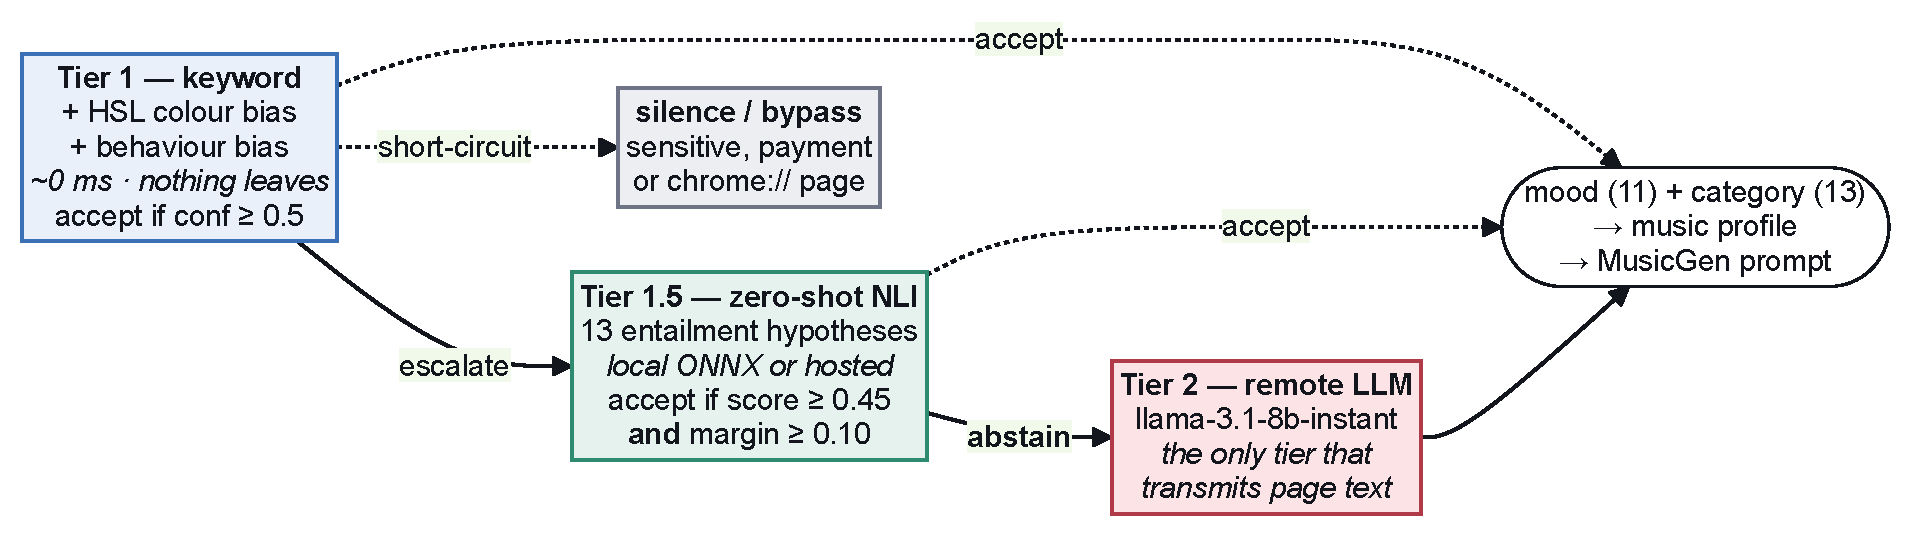
\includegraphics[width=\textwidth]{figures/cascade.pdf}}
\caption{The three-tier classifier. Each tier carries its own acceptance
condition; a tier that cannot meet it escalates. Tier 1.5 is an entailment
model and can therefore \emph{abstain}, which is what makes its two thresholds
a continuous dial between accuracy and exposure rather than a fixed operating
point. Tier 2's remote LLM always transmits page text off the device, and so
does Tier 1.5 as shipped here (hosted backend, not the local ONNX
alternative) -- both are unreachable for pages the sensitive check has
already short-circuited.}
\label{fig:cascade}
\end{figure*}

\textbf{Tier 1, keyword heuristic.} A keyword map over title, description and
cleaned text produces a category. The mood distribution blends the keyword
score with an HSL colour bias, in which saturation and lightness shift valence
and arousal, and a behaviour bias, in which scroll and cursor velocity shift
arousal. If the resulting confidence reaches 0.5 the pipeline stops here, at
essentially zero cost and with nothing leaving the device. The tier is skipped
by construction for non-English pages, which is the single largest known gap in
the design.

\textbf{Tier 1.5, zero-shot NLI with abstention.} On escalation the cleaned
text is scored as an NLI premise against thirteen category hypotheses. The tier
returns a label only if the top score is at least 0.45 \emph{and} its margin
over the runner-up is at least 0.10; otherwise it abstains and escalates. Two
backends exist: a hosted entailment endpoint, and a fully local quantised ONNX
export that runs in the extension's own worker, which makes a zero-exposure
configuration possible at some accuracy cost.

\textbf{Tier 2, remote LLM.} A hosted instruction-tuned model with a structured
JSON response, an eight-second timeout, and a fall-back-to-tier-1 path on any
failure. This is not the only tier that transmits page text -- Tier 1.5's
hosted backend does too, as shipped -- but it is the tier whose reaching
fraction this paper calls the exposure rate specifically.

\textbf{Profile and prompt.} The committed mood is mapped to a music profile,
comprising tempo, key, energy, valence, intensity, instrument list, timbre,
reverb, ambience, style and dynamics, and thence to a generator prompt. For the
\emph{focused} mood this yields, in part: ``lo-fi study, minimal electronic,
deep focus. Instruments: piano, minimalist synth, light percussion, bass drone.
Key: D minor, 88 BPM. No vocals. Seamlessly loopable. Instrumental only.''

\textbf{The confidence window.} A newly classified mood does not take effect
immediately; it must remain stable for five seconds before a transition is
committed, so that scrolling through a link-heavy page or a brief detour does
not cause the music to lurch. As Section \ref{sec:res-latency} shows, this is
by far the largest term in the end-to-end wall clock, and it is a design
parameter rather than an implementation limitation -- but it is an unexamined
one: no sweep of this value against false-commit rate or perceived
responsiveness has been run, so there is no stated reason it is five seconds
rather than three or ten, only that it is the value shipped.

\subsection{Feature D: generation, loop synthesis and caching}

Feature D is an HTTP service with a five-stage pipeline, shown in
Fig.~\ref{fig:featured}: validate, prompt, generate, post-process, cache.
Validation fills every missing field with a default, so a malformed profile
degrades rather than fails.

\begin{figure*}[t]
\centerline{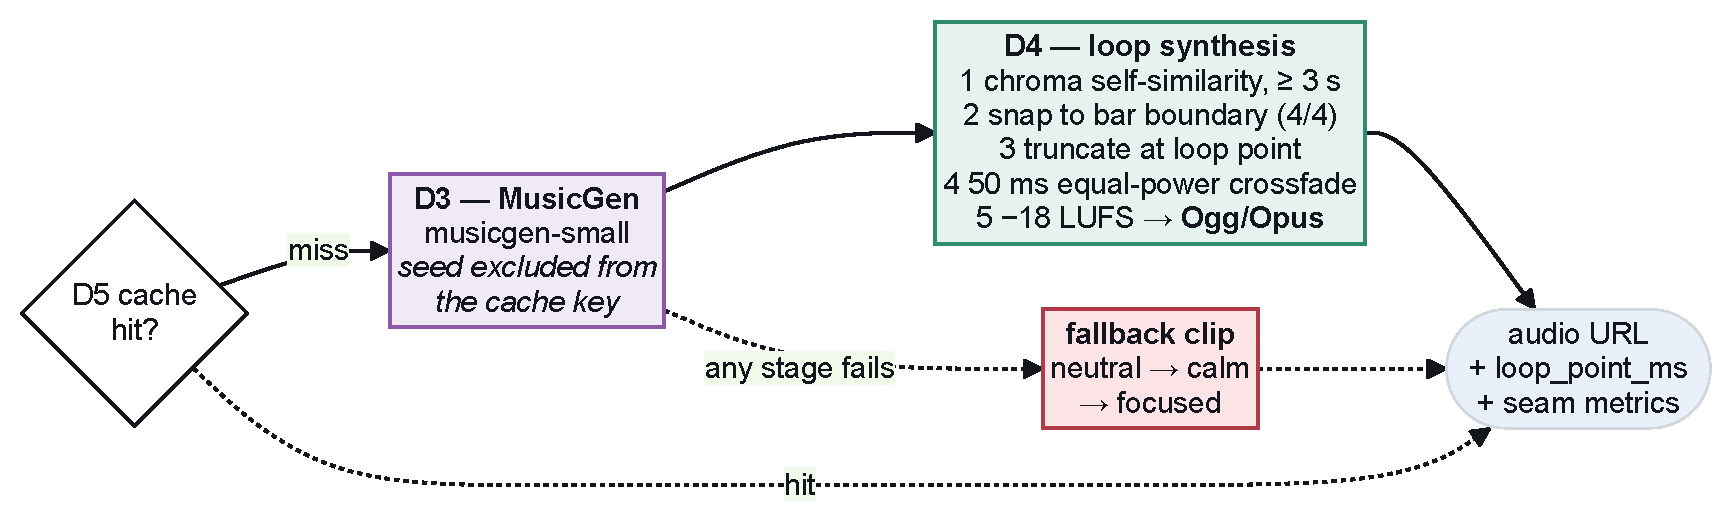
\includegraphics[width=\textwidth]{figures/featured.pdf}}
\caption{Feature D. The cache is consulted before the generator, and any stage
failure diverts to a pre-generated per-mood clip rather than an error. The D4
box is the loop-synthesis stage that converts a one-shot generator output into
material that repeats; step 3 is where roughly half the generated audio is
discarded, and step 5 is where the container choice, rather than the crossfade,
is what actually makes the loop gapless.}
\label{fig:featured}
\end{figure*}

\textbf{Loop synthesis.} The generator produces a one-shot clip, not a loop.
Chroma features are computed and a vectorised self-similarity curve
\cite{foote} is evaluated over candidate loop lengths, excluding anything
shorter than three seconds -- an engineering default with no documented
derivation, unlike the cosine thresholds in Section
\ref{sec:arch} which the implementation itself frames as tuning starting
points. The best candidate is snapped to a bar boundary
inferred from beat times \cite{ellis, librosa} under a 4/4 assumption, since
true downbeats are not available. The clip is truncated at the loop point, and
its head and tail are blended with a 250 ms equal-power crossfade (Section
\ref{sec:res-loop} justifies this width against the 50 ms default used to
produce this paper's other seam measurements) so that the loop is continuous
in energy across the seam. Loudness is normalised to
$-18$ LUFS \cite{ebu128} and the clip is exported as Ogg/Opus \cite{opus}
rather than MP3. That last choice is not aesthetic: an MP3 encoder pads the
stream, and the padding is audible as a gap on every loop iteration. The
container, not the crossfade, is what makes the loop gapless -- an inference
from Opus's documented format properties \cite{opus} rather than something
this pipeline measures directly (\S\ref{sec:res-loop} states the gap
precisely). The $-18$
LUFS target is not a departure from \cite{ebu128} by oversight: the
citation is for R128's integrated-loudness measurement algorithm, which
this pipeline implements to compute every LUFS figure reported in Section
\ref{sec:res-loop}, not for its $-23$ LUFS broadcast target, which is
calibrated for dialogue-forward television content rather than background
music in an interactive application. $-18$ LUFS sits closer to targets
common for streaming and ambient background audio; no further
target-selection rationale beyond this is recorded in the implementation.
The service also
computes a diagnostic seam discontinuity, the RMS energy and spectral-centroid
differences across the seam, both before and after the crossfade; this is the
objective measure reported in Section \ref{sec:res-loop}.

\textbf{Cache.} Requests are keyed on mood, style and key exactly, on energy,
valence and arousal to one decimal place, on a three-way tempo bucket, a
two-second duration bucket, and the export codec, so that a codec change
invalidates the cache automatically. The generation seed is deliberately
excluded: retries use fresh seeds, and including it would defeat caching
entirely. A pre-warm grid of ninety-nine mood, style and tempo-bucket
combinations is generated ahead of time.

\subsection{Feature C: extension shell and playback}

Playback lives in an offscreen document. Two alternating decks over raw audio
buffer sources, rather than a higher-level player abstraction, are required so
that loop start and end points can honour the detected loop point. They feed
four independent gain stages in series, for crossfade, user volume, ducking and
mood fade, so that un-ducking cannot erase a mood fade in progress, and then an
equaliser, reverb and analyser chain.

\textbf{Fallback-then-swap} is the mechanism that hides generation latency. On
a committed mood the client issues a request for the pre-generated fallback
clip and a generation request in parallel. The fallback clip, correct in mood
and generic in content, begins playing immediately; when generation completes,
the generated clip is crossfaded in on the second deck. One abort controller
per request means a new mood cancels a stale generation rather than letting it
arrive late and overwrite a now-incorrect track.

\textbf{Restraint.} Three behaviours are deliberate refusals to produce output.
Pages classified as sensitive, covering crisis, grief, self-harm and violence,
produce silence, and their text is short-circuited before either LLM tier.
If the active tab is itself audible the extension mutes, and if a background
tab is audible it ducks, so that it never competes with media the user chose.
Payment, banking and checkout pages, and all browser-internal URLs, are
bypassed entirely.

\textbf{Telemetry} is a local-only ring buffer. Every URL is hashed with
SHA-256 before storage and nothing leaves the machine unless the user
explicitly exports it. This bound is thinner than it sounds: URLs are
public, so a bare SHA-256 hash is dictionary-recoverable against a modest
precomputed table of common ones -- the guarantee is that plaintext never
leaves the device, not that a stored hash cannot be reversed to the URL it
came from. An HMAC keyed with a per-install local secret, rather than a
bare hash, would close this gap without changing what leaves the device;
it has not been implemented here.

% ===========================================================================
\section{Results and Discussion}
\label{sec:results}
% ===========================================================================

\subsection{Evaluation design and provenance}

Five studies: S1 (systems benchmark), S2 (tier ablation), S3 (audio/loop
quality), S4 (within-subjects perceptual), S5 (in-the-wild). S1, the
objective half of S3, the retrieval baseline and restraint audit are
reported here; S4/S5 require ethics approval not yet obtained.
\textbf{Corpus.} 260 pages (255 captured): 182 general, 15
vocabulary-mismatch, 15 non-English, 15 mixed-genre, 12 sensitive, 15
sensitive near-miss, 6 bypass. Four page counts appear across this paper
and do not share one arithmetic, so here is the reconciliation rather than
four numbers that look like a typo of each other: 260 is the S2 corpus's
target size (matches the slice breakdown just given); 255 is what the
extraction benchmark actually captured (\texttt{s2\_corpus.json}: 255
captured, 2 navigation failures, 3 bypassed-as-expected outcomes, summing
to 260); 254 is 260 minus the 6-page bypass slice, computed directly from
\texttt{s2-ablation.json}'s per-page records (6 of its 260 entries carry no
\texttt{true\_category}, matching the bypass count exactly) -- a different
snapshot than the one behind ``255 captured,'' not an arithmetic slip,
since 255 minus 6 does not reconcile to 254 and 260 minus 6 does; and 208
is not a further reduction of either -- it is the full per-page record
count of \texttt{s2-ablation-real.json}, a separate results file (built
against \texttt{s2\_corpus\_annotated.json} on a different contributor's
machine) used specifically for \S\ref{sec:res-classification}'s re-scoring
paragraph. The four numbers name three different corpus snapshots, not one
pipeline with three clean exclusion steps. \textbf{Annotator wellbeing.}
Three annotators labelled all 12 sensitive and 15 sensitive-near-miss
pages, covering crisis and self-harm content, as part of this task; no
informed-consent, opt-out, or debriefing process for that specific
exposure is recorded anywhere in this project's materials, and none
should be assumed present. That is a gap in how this annotation was run,
not a detail omitted from the writeup, and it should be closed before any
further annotation of this kind is asked of anyone.
\textbf{Hardware.} A single CPU laptop for every figure except the
cache-cold generation results (Apple Silicon, MPS backend, \S\ref{sec:res-latency}).
\textbf{Deployment status.} Web2Music has
not been submitted to the Chrome Web Store or otherwise distributed: the
README's only installation path is Chrome's developer-mode ``Load
unpacked'' against a locally built \texttt{ui/dist/}, itself requiring a
local \texttt{services/classify} instance and manually generated fallback
clips first, and Chrome dropped command-line unpacked loading from stable
at v137 -- there is no public-facing artefact a non-technical user could
install. This does not excuse the sensitive-content detector's 65.5
percent false-negative rate (\S\ref{sec:res-audit}); it narrows who is
currently exposed to it to developers running the extension locally, not
the public the restraint policy is nominally written for.

\textbf{Availability.} The system's source code, the extraction and
generation pipelines, the analysis scripts behind every table and figure
in this paper, and the corpus of extracted page descriptors are available
at \url{https://github.com/AyushK0808/web2music}.

\subsection{Annotation agreement and human ceiling}
\label{sec:res-agreement}

Three independent annotators labelled all 255 pages for category (13-way),
mood (11-way, a preference not a fact) and sensitivity (binary); Table
\ref{tab:agreement} reports bootstrap Krippendorff's-alpha and
leave-one-annotator-out ceiling for each.

\begin{table}[t]
\caption{Inter-annotator agreement, three annotators, 255 units.}
\label{tab:agreement}
\begin{center}
\scriptsize
\begin{tabular}{lcccc}
\toprule
\textbf{Label} & \textbf{$\alpha$} & \textbf{95\% CI} & \textbf{Ceiling} & \textbf{Gate} \\
\midrule
Category  & 0.635 & [0.578, 0.689] & 0.621 & below 0.667 \\
Mood      & 0.195 & [0.149, 0.238] & 0.174 & below 0.667 \\
Sensitive & 0.419 & [0.301, 0.530] & 0.775 & below 0.667 \\
\bottomrule
\end{tabular}
\end{center}
\end{table}

All three label sets fall below the 0.667 minimum the plan sets for drawing
conclusions, and none reach the 0.80 threshold for good agreement. Per that
same policy, we report this as a finding rather than treat it as a defect to
fix by re-annotating, and the mood result is the more important of the two to
read this way. At $\alpha=0.195$, three annotators working independently from
the same instructions are close to chance-level agreement on which of eleven
moods a page calls for. The system's primary output is an eleven-way mood.
That three humans cannot agree on it is not a footnote to the mood
classifier's accuracy; it is evidence about the task itself, and it says the
task, as specified, may not have a single defensible answer per page. Category
agreement (0.635) is closer to usable but still short of it.

Both ceilings in Table \ref{tab:agreement} sit below their own label's
$\alpha$ -- 0.621 against 0.635 for category, 0.174 against 0.195 for
mood -- which looks like an error but follows from what the two statistics
actually measure. The ceiling is a strict, conservative hit rate: does the
held-out annotator's label exactly match the majority of the other two,
with any tie between those two others counted as a miss rather than a
partial credit, by deliberate design so the ceiling is never inflated. With
only three annotators, ``majority of the other two'' is frequently a tie,
and every tie is a guaranteed miss regardless of how close the three labels
actually were. $\alpha$, by contrast, is a chance-corrected coefficient
averaged continuously across all pairwise comparisons, with no majority
requirement and no all-or-nothing penalty for a near-miss. A ceiling built
from strict, tie-punished binary hits has no guaranteed ordering against a
smoother, chance-corrected coefficient, and sensitivity's ceiling sitting
\emph{above} its own $\alpha$ later in this table is the same asymmetry
running the other way.

To ask whether that disagreement is a fine-grained labelling problem rather
than a disagreement about the underlying affect, we collapsed the eleven mood
labels onto Russell's valence-arousal circumplex two different ways and
recomputed $\alpha$ on the same three annotators' raw labels under each. We
name the four quadrants by axis sign throughout -- positive-valence/
high-arousal, negative-valence/high-arousal, negative-valence/low-arousal,
positive-valence/low-arousal -- rather than by an exemplar mood word, because
an exemplar can end up outside its own quadrant and read as an error rather
than as the finding it is.

The first mapping uses this system's own per-mood valence hint and BPM-range
midpoint, the same encoding used elsewhere in the pipeline, with a median
split. It gives $\alpha=0.121$, 95\% CI [0.057, 0.186] -- lower than the
eleven-way figure, not higher -- under heavily skewed membership: the
positive-valence/high-arousal quadrant alone accounts for 466 of 697
annotator judgements (66.9 percent).

Because that mapping tests this system's own taxonomy's geometry rather than
Russell's, we repeated the collapse using the NRC Valence-Arousal-Dominance
lexicon's published word-level norms~\cite{nrcvad}, splitting each axis at
the lexicon's own 0--1 scale midpoint, 0.5, not a median fit to these eleven
words specifically. (One mood word, ``focused,'' has no direct entry; we
substitute its lemma, ``focus.'') Under these norms, no mood word falls in
the negative-valence/high-arousal quadrant at all, including the word
``tense'' itself, which the norms rate as low-arousal -- a coverage gap in an
eleven-word taxonomy built without reference to a circumplex, not an
artefact of the mapping. Membership across the three occupied quadrants is
289, 222 and 186 of 697 judgements: less skewed than the first mapping, but
the largest quadrant still holds 41.5 percent. This mapping gives
$\alpha=0.300$, 95\% CI [0.231, 0.365].

As a sanity check on the recomputation itself, we re-ran the identical
procedure on the original eleven-way labels, with no quadrant collapse. It
returns exactly 0.195, matching the raw figure reported above. This confirms
the collapse step, not a bug in the recomputation, is what moves the number
under either mapping.

The two mappings disagree about which way coarsening moves agreement: the
system's own geometry makes it worse, published norms make it nearly double.
Both start from the same three annotators' raw labels; only the placement of
eleven words on two axes differs. That the answer flips with the mapping is
itself informative, not a nuisance to resolve before reporting a number -- it
means quadrant-level agreement for this taxonomy is sensitive to exactly
where the words sit, a second and independent argument that the affective
target is underdetermined, on top of whichever $\alpha$ is closer to correct.
A boundary check on the NRC-VAD placements sharpens this: five of the eleven
words -- nostalgic, curious, tense, uplifting and neutral -- sit within 0.1
of a 0.5 split on at least one axis, so nearly half the taxonomy's quadrant
memberships are close calls rather than clear regions, and a different norm
source could plausibly move several of them to a different quadrant.

\textbf{Post-hoc mood re-collapse at 3-way and 2-way.} The two circumplex
mappings above test whether a different geometry over the same eleven words
changes agreement; a separate question is whether simply asking for fewer
buckets does, independent of any circumplex mapping. Collapsing to 3-way
arousal buckets (calm $\leftarrow$ \{calm, sad, nostalgic\}, neutral
$\leftarrow$ \{focused, curious, neutral\}, energetic $\leftarrow$ \{joyful,
energetic, uplifting, tense, dark\}) and to 2-way valence buckets (positive
$\leftarrow$ \{calm, focused, joyful, energetic, curious, uplifting,
neutral\}, negative $\leftarrow$ \{sad, dark, tense, nostalgic\}) does not
clear the gate at either resolution: $\alpha=0.281$ [0.204, 0.353] at 3-way
and $\alpha=0.259$ [0.125, 0.383] at 2-way, against 0.195 at 11-way -- all
three computed with the same coincidence-matrix \texttt{nominal\_alpha()}
and page-level bootstrap the eleven-way figure uses, over all 255 units and
the three annotators' raw per-page judgements. Coarsening does not rescue
mood under this collapse either: even a binary positive/negative split
leaves three annotators short of the 0.667 minimum. One thing does move
sharply with granularity and is worth flagging on its own: the
leave-one-annotator-out ceiling rises from 0.174 (11-way) to 0.402 (3-way)
to 0.788 (2-way), while $\alpha$ does not follow it -- coarsening a label
space inflates the ceiling a classifier would be scored against largely by
construction (fewer buckets means more accidental agreement), not because
annotators have started agreeing on anything more meaningful. A future
switch to a coarser mood target should not cite the higher ceiling alone as
justification. Read together with the circumplex collapse above, three
independent coarsening strategies -- two geometric, one a flat re-bucketing
-- all fail to clear the usability gate, which is a stronger claim than any
one of them alone: mood is underdetermined by page content at every
resolution tested here, not just the eleven-way one this system reports.

Sensitivity is the most consequential label for the system's abstention
policy, and its two statistics diverge: $\alpha=0.419$ is below threshold,
while the leave-one-out human ceiling is the highest of the three (0.775).
This is consistent with the label's skew — 219 of 250 resolved units (87.6\%)
are majority-labelled not-sensitive — since chance-corrected agreement
statistics are depressed by a lopsided marginal distribution even when raw
annotator agreement is substantial, precisely because chance agreement is
already high under that skew. The two numbers should be read together rather
than either alone: annotators mostly agree on individual pages, but that
agreement is not distinguishable enough from chance under $\alpha$'s
definition to clear the plan's own bar. Any classifier-accuracy claim drawn
from this corpus, including the tier-ablation rebuild in Section
\ref{sec:res-classification}, must be interpreted against these ceilings
rather than against a naively perfect one.

\subsection{Extraction cost}
\label{sec:res-extraction}

Table \ref{tab:extraction} reports descriptor construction over 105 real
websites in a Playwright-driven Chromium.

\begin{table}[t]
\caption{Page descriptor extraction cost, 105 real sites, CPU laptop. The embedding
stage was stubbed in this run; see the caveat in the text.}
\label{tab:extraction}
\begin{center}
\scriptsize
\begin{tabular}{lrr}
\toprule
\textbf{Stage} & \textbf{p50 (ms)} & \textbf{p95 (ms)} \\
\midrule
Text extraction (boilerplate removal) & 11.0 & 55.5 \\
Colour histogram (800 elements) & 3.9 & 9.7 \\
Readability (Flesch) & 1.5 & 7.1 \\
Behaviour snapshot & 0.13 & 0.30 \\
Embedding (stubbed) & 1.2 & 2.6 \\
Vector-store similarity search & 50.3 & 1222 \\
\midrule
\textbf{Total descriptor construction} & \textbf{85.9} & \textbf{1303.6} \\
\midrule
Forced layouts (count) & 21 & 100 \\
Layout duration (ms) & 151.3 & 620.6 \\
Text coverage (extracted / visible words) & 0.808 & --- \\
\bottomrule
\end{tabular}
\end{center}
\end{table}

The descriptor is cheap at the median, 86 ms against a median navigation time
of 1989 ms on the same pages, and it is scheduled at idle so it does not
contend with page load. The cost is, however, strongly skewed: the 95th
percentile is fifteen times the median and the maximum is 5.1 s, driven almost
entirely by the vector-store similarity search, whose 95th percentile of 1222
ms sits against a median of 50 ms on pages where the store has grown large.
Boilerplate removal retains a median of 80.8 percent of visible words, which is
the figure that matters for downstream classification quality.

The embedding stage in this run was stubbed, so
its 1.2 ms median is harness overhead rather than MiniLM inference; the total
above should be read as covering everything except the embedding.

The in-browser embedding cost has since been measured directly, and the
result is two findings rather than one number, neither of which belongs in
Table \ref{tab:extraction} itself: this was a separate run against a real
Chrome, not the Playwright-instrumented one above, and the latency finding
below is an artefact of this benchmark's own methodology rather than a
property of the system, for reasons stated with it.

First, real MiniLM inference did not run on every site. Loading it requires a
cross-origin fetch to the Hugging Face Hub for the model config, tokenizer and
weights, and a real site's own Content-Security-Policy can block that
outright -- confirmed directly on this benchmark's Wikipedia-family sites,
whose \texttt{connect-src} allowlist admits dozens of Wikimedia and partner
domains but not \texttt{huggingface.co}, producing a same-shaped
\texttt{Refused to connect} console error on every one of them. Across the
full site list, 103 of 105 sites completed navigation (the other two are
unrelated: an execution-context-destroyed and a navigation timeout, neither
touching embedding) and 31 of those 103 failed the embedding stage, a rate
consistent with the same CSP mechanism though not individually confirmed for
every failing site. Read as a lower bound on deployability: at least 69.9
percent of real sites permit in-browser embedding as built, entirely
independent of anything this system controls, and the remaining share is a
real constraint on the design rather than a bug in it.

Second, on the sites where it succeeded, per-page latency (mean 7.0 s, median
9.0 s, 95th percentile 15.7 s) is dominated by a cold model download, not
inference, and overstates what a real user would experience. Each site in
this benchmark is a fresh page at a different origin, and browser cache
storage is origin-scoped, so nothing carries over between sites; the one
repeated domain in the site list (\texttt{smashingmagazine.com}, visited once
near the start and again at the end) fell from 10.1 s to 0.4 s on the second
visit, a twenty-five-fold difference attributable entirely to the cache. The
real extension does not re-pay this cost per page the way this benchmark
does: the embedding model loads once, into the extension's own persistent
offscreen-document origin, not the origin of whatever page the user is
reading, so the number this methodology cannot measure directly is closer to
the 0.4 s repeat-visit figure than to the multi-second first-visit ones
reported above.

Separately from the embedding measurement above, the six stage medians in
Table \ref{tab:extraction} sum to 68.0 ms, not the reported 85.9 ms total:
percentiles are not additive across independent stages even when the
underlying work is, since each stage's own tail is measured separately from
the sum's tail, so the gap is an artefact of reporting percentiles rather
than a missing stage. The 151.3 ms median layout duration is a different
quantity again, not a component of either figure: it is Chrome's own
cumulative layout counter since the page was created, covering layout work
from navigation and initial render as well as anything the descriptor
construction itself triggers, so it is scoped to the whole page session
rather than to the descriptor-construction code specifically.

\subsection{Which signals earn their cost}
\label{sec:res-signal-ablation}

A per-signal offline ablation (255 pages): category never changes, decided
by text alone — measurable against a real ceiling (0.621,
\S\ref{sec:res-agreement}), so this is a genuine finding. Removing
behaviour or the embedding changes the descriptor's own predicted mood
label on zero pages; removing colour changes it on 7.5 percent, text-alone
on 10.2 percent.

These mood counts are self-consistency against no ground truth at all —
whether removing a signal flips the offline rule's own output — not
accuracy. Three annotators agree on mood at only $\alpha=0.195$
(\S\ref{sec:res-agreement}), close to chance, so there is no validated
target for a signal to move toward; a signal perturbing an unvalidated
label on 7.5 percent of pages has not been shown to move anything a person
would recognise as better mood-matching. Read this as bounding what colour
perturbs in the offline rule's own arithmetic, not as showing colour is
the signal worth keeping for mood — on the mood side, the pathway these
counts are taken over is unvalidated end to end, and no per-signal
movement count changes that. This ran offline (keyword default, not
either model tier), so it bounds rather than measures colour's
contribution live; a live-tier repeat remains future work
(\S\ref{sec:limitations}) and would still inherit the mood-validity gap
above.

\subsection{Generation latency and its failure modes}
\label{sec:res-latency}

Table \ref{tab:d-latency} reports 144 requests: five distinct modes, so a
mean would describe nothing that ever happened.

\begin{table}[t]
\caption{Generation service latency by request class, and server-side
stage times for the same run, $n=144$, CPU laptop. Nearest-rank
percentiles.}
\label{tab:d-latency}
\begin{center}
\scriptsize
\begin{tabular}{lrrrr}
\toprule
\textbf{Request class} & \textbf{n} & \textbf{p50 (ms)} & \textbf{p95 (ms)} & \textbf{max (ms)} \\
\midrule
Fallback endpoint & 33 & 7 & 153 & 154 \\
Cache hit & 93 & 2{,}090 & 2{,}114 & 2{,}169 \\
Cache miss (generated) & 3 & 139{,}318 & 207{,}468 & 207{,}468 \\
Generation to fallback & 3 & 126{,}733 & 239{,}516 & 239{,}516 \\
Client timeout (300 s) & 12 & 300{,}009 & 300{,}018 & 300{,}018 \\
\midrule
\textbf{Server stage} & \textbf{n} & \textbf{p50 (ms)} & \textbf{p95 (ms)} & \\
\midrule
D1 validate & 99 & 0 & 0 & \\
D2 prompt build & 6 & 0 & 0 & \\
D3 generate & 3 & 134{,}673 & 202{,}828 & \\
D4 post-process (loop, export) & 3 & 504 & 516 & \\
D5 cache check & 99 & 2{,}082 & 2{,}100 & \\
D5 save & 3 & 2{,}063 & 2{,}077 & \\
Unaccounted (queue, transport) & 99 & 6 & 82 & \\
\bottomrule
\end{tabular}
\end{center}
\end{table}

The fallback clip is served in a median of 7 ms against 139 s for
generation (Table \ref{tab:d-latency}, which also attributes time to
server stages): fallback-then-swap is the only reason the system is usable
on CPU, confirming that it keeps time-to-first-audio within the latency
budget. Fig.~\ref{fig:f1} shows the timeline,
Fig.~\ref{fig:f2} shows generation scaling with duration, and
Fig.~\ref{fig:f3} the request path under concurrency.

\begin{figure}[t]
\centerline{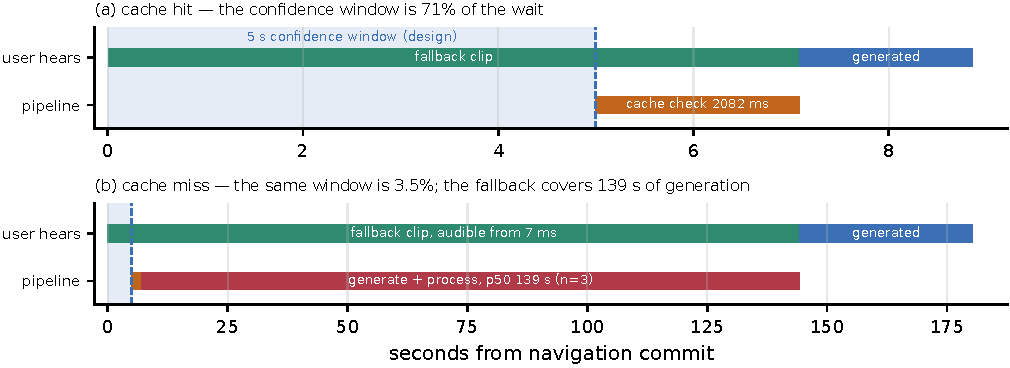
\includegraphics[width=3.42in]{figures/f1.pdf}}
\caption{Server-side timeline: navigation to first sound to generated swap,
with the five-second confidence window shaded as a design interval rather than
a cost. Server-side generation path only; client-side extraction, decision and
decode segments are measured separately (Section~\ref{sec:res-e2e-latency}).}
\label{fig:f1}
\end{figure}

\begin{figure}[t]
\centerline{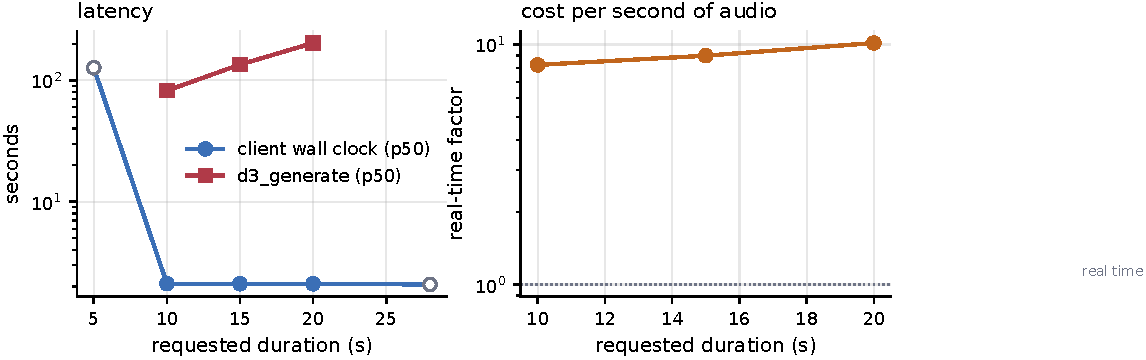
\includegraphics[width=2.24in]{figures/f2.pdf}}
\caption{Generation latency against requested clip duration, with the
real-time-factor line. Open markers are duration cells in which no request
reached the generator; the real-time-factor line is drawn only where measured.}
\label{fig:f2}
\end{figure}

\begin{figure}[t]
\centerline{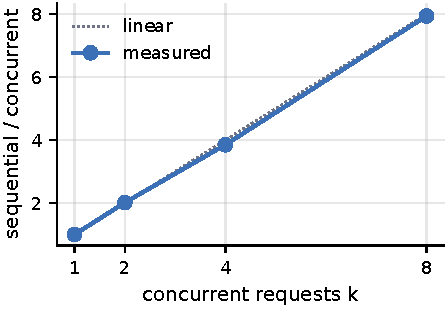
\includegraphics[width=\columnwidth]{figures/f3.pdf}}
\caption{Cache-hit request throughput against concurrency -- not generator
throughput. Every request in this sweep was a cache hit, so the
near-linear scaling describes the request and cache path only; reporting
it as generator batching would require a cold-cache re-run, which this
figure is not.}
\label{fig:f3}
\end{figure}

Four qualifications belong with these tables. First, only three of 144 requests
actually invoked the generator, because the pre-warm grid was already populated
when the run executed; the generation percentiles therefore rest on $n=3$ and
their confidence intervals are correspondingly wide, with a 95 percent interval
on the median of 86.8 s to 207.5 s. The D2 prompt-build count of six, not three, is not a discrepancy: the
server builds a prompt on every cache miss before attempting generation, but
only records a D3 timing on success. The other three cache misses are the
three ``Generation to fallback'' events in Table \ref{tab:d-latency} --
MusicGen's own retry budget was exhausted on those calls and the server fell
back to a pre-generated clip, so a prompt was built (D2) but no D3 timing
exists to report. Second, there is no cold-cache column in this table: the
run's cold section produced 33 cache hits and no misses, and measuring
cold-cache behaviour requires flushing the cache before the section -- the
dedicated cold-cache runs below do exactly that. Third,
8.3 percent of requests, twelve of 144, hit the client's 300 s timeout; these
are reported as their own row rather than dropped from the percentiles, and a
one-in-twelve timeout rate is itself a finding about the viability of CPU-only
deployment -- not a tail-latency footnote, and one this paper does not
otherwise account for or attribute a cause to. \textbf{Discussion.}
Fallback-then-swap makes a 139 s generator feel immediate, at the cost of the
first seconds being generic — nearly invisible, since a listener cannot miss
a clip they never heard. The dominant wall-clock term is thus the
five-second confidence window we chose (\S\ref{sec:arch}) and never swept,
not the model.

\textbf{The 2.08 s cache check was a bug, not a cost, and it is now fixed.}
\texttt{cache\_key} carries a \texttt{UNIQUE} constraint, which Postgres
indexes automatically, so the lookup itself was never the bottleneck. The
cause was that \texttt{check\_cache} and \texttt{save\_to\_cache} each
opened a fresh database connection and closed it immediately after a
single query, on every request, with no pooling at all --
\texttt{d5\_cache\_local.py}'s three call sites opened a brand-new
psycopg2 connection to Postgres and closed it again on every single call,
instead of reusing one. Replacing this with a lazily-initialised,
pooled connection
(\texttt{psycopg2.pool.ThreadedConnectionPool}, minconn=1, maxconn=10),
verified for correctness (MISS $\to$ INSERT $\to$ HIT with the right row)
against a real database, not a mock, and separately verified against 27
real cache-hit requests through the live service, reduced the step to a
p50 of 2.1 ms (p95 4.3 ms) on the verification host and to 8 ms p50 / 41 ms
p95 (max 391 ms, the pool's first cold-start borrow) across 30 real
cache-cold requests on a second, independent machine below -- roughly
three orders of magnitude either way. The exact original 2082 ms figure
itself did not reproduce on any benchmarking host used since: a fixed
$\approx$2 s-per-new-connection cost is the signature of the
well-documented Docker-Desktop-on-Windows ``localhost'' IPv6-then-IPv4
resolution stall, consistent with the Windows development paths visible
elsewhere in the project's run artefacts, and not a mechanism a native
Linux loopback or Apple Silicon host reproduces. Either way, the fix
removes the cause: nothing in \texttt{check\_cache} or
\texttt{save\_to\_cache} opens a new connection per call any more, on any
host tested since. Table \ref{tab:d-latency}'s D5/cache-hit rows describe
the pre-fix build and remain unreplaced at that scale on the original CPU
laptop; the cache-cold results below, from two independent post-fix runs
on Apple Silicon, are current.

\textbf{Cache-cold generation latency on a second machine.} Table
\ref{tab:d-latency}'s ``Cache miss (generated)'' row was $n=3$ -- too few
for a percentile to mean anything. Two independent post-fix runs since
close this gap, both on Apple Silicon (MPS backend) rather than the CPU
laptop the rest of this paper's absolute-latency numbers come from -- a
second, separate hardware point (\S\ref{sec:limitations}), not a
replacement for Table \ref{tab:d-latency}'s CPU figures, and the two
should not be read as one population. The first, a tightly-controlled
$n=30$ run at a single mood (\emph{calm}) with every request confirmed a
genuine cache miss and zero failures, gives a median wall time of 72.1 s
(Table \ref{tab:d-latency-cold}); D3 generation is completely dominant, as
on CPU, at 71.5 s of that median, with every other stage summing to under
a second combined at p50. The second, a wider $n=110$ run across the full
mood set with a genuinely cold cache, gives a closely consistent median of
72.4 s (p95 119.4 s, max 183.2 s) and adds two findings the narrower run
could not surface: median generation time varies nearly twofold by mood
alone, from 48.5 s (\emph{uplifting}) to 99.0 s (\emph{dark}), at the same
requested duration and token budget, so prompt content, not just length,
measurably affects generation time; and, under genuine concurrent load at
eight simultaneous requests, four of eight individually exceeded the 300 s
client timeout before the queue could clear them -- the same one-in-twelve
timeout finding from the CPU run above, now reproduced on different
hardware under directly-provoked contention rather than incidentally
encountered. Both cache-cold runs land at 72 s, comfortably faster than
the CPU laptop's 139 s median for the same target duration, consistent
with MPS acceleration over CPU-only inference and not a correction to the
CPU number; \texttt{torch.compile} does not apply on either run
(CUDA-only in \texttt{d3\_generate.py}), so both are plain-eager MPS
inference. The narrower run's D5 cache-check timings (8 ms p50 / 41 ms p95,
against the 2082 ms pre-fix figure) additionally confirm the fix holds
end to end under real traffic on a second machine, using a checked-out
copy of the patched \texttt{d5\_cache\_local.py} verified byte-identical
to the version described above, not a drifted or partially-applied copy
-- confirmation the fix removes whatever the original cost was, on every
machine tested so far, though the two runs' hardware and OS both differ
from the CPU laptop, so together they cannot by themselves distinguish
the Docker-Desktop-on-Windows stall theory above from any other
explanation for the original number.

\begin{table}[t]
\caption{Cache-cold generation latency, Apple Silicon (MPS backend), single
mood (\emph{calm}), $n=30$, all requests confirmed cache misses, zero
failures. Nearest-rank percentiles.}
\label{tab:d-latency-cold}
\begin{center}
\scriptsize
\begin{tabular}{lrrr}
\toprule
\textbf{Stage} & \textbf{p50 (ms)} & \textbf{p95 (ms)} & \textbf{max (ms)} \\
\midrule
Wall clock (total) & 72{,}129 & 105{,}921 & 173{,}344 \\
D1 validate & 2 & 15 & 39 \\
D2 prompt build & 0 & 4 & 5 \\
D3 generate & 71{,}504 & 104{,}859 & 171{,}495 \\
D4 post-process (loop, export) & 896 & 3{,}487 & 5{,}864 \\
D5 cache check & 8 & 41 & 391 \\
D5 save & 44 & 225 & 564 \\
Unaccounted (queue, transport) & 44 & 93 & 103 \\
\bottomrule
\end{tabular}
\end{center}
\end{table}

\textbf{The duration-scaling question no longer rests on $n=3$ -- but on
different hardware.} A dedicated sweep -- five requested durations, three
repeats each, every request forced to a live cold generation with a fresh
nonce -- has since been run on the same Apple Silicon (MPS) machine, not
the CPU laptop that produced the 139 s figure reported everywhere else in
this paper. Its 28 s cell measures a median cold generation time of 48.9 s,
roughly a third of 139 s: consistent with MPS acceleration over CPU-only
inference, not a correction to the CPU number, and the two should not be
compared as if they measured the same thing. Every other figure in this
paper that reports absolute generation latency -- the 139 s headline, Table
\ref{tab:d-latency} -- remains the CPU-laptop measurement and is
unaffected. What this sweep speaks to, on its own hardware, is the
\emph{shape} of the duration-latency relationship, not its absolute
CPU-laptop magnitude, and it is reported alongside the clip-length sweep
in Section~\ref{sec:res-loop}, which shares its methodology and backend.

\subsection{Client-side (in-browser) latency}
\label{sec:res-e2e-latency}

An end-to-end Playwright harness drives the built extension against eleven
synthetic fixture pages; the generation service was stubbed at
139{,}894 ms to isolate the client-side critical path. 54 of 55 page
loads reached audible playback; the one that did not is an unresolved
1.8 percent failure, not a rounding artefact -- it has not been
root-caused, and every table below reports $n=54$, not 55.

\begin{table}[t]
\caption{End-to-end client-side latency, $n=54$ page loads, nearest-rank
percentiles.}
\label{tab:e2e-latency}
\begin{center}
\scriptsize
\begin{tabular}{p{3.3cm}rrr}
\toprule
\textbf{Stage} & \textbf{p50 (ms)} & \textbf{p95 (ms)} & \textbf{max (ms)} \\
\midrule
Nav $\to$ page data (extraction + idle/debounce) & 856 & 1{,}217 & 1{,}272 \\
\quad of which extraction itself & 464 & 833 & 865 \\
Classifier decision, per call & 16 & 28 & 32 \\
Generation round trip (stubbed) & 139{,}920 & 139{,}933 & 139{,}951 \\
Fetch + decode + crossfade start & 38 & 74 & 86 \\
Nav $\to$ audible (wall clock, incl. window) & 6{,}859 & 11{,}279 & 11{,}291 \\
\bottomrule
\end{tabular}
\end{center}
\end{table}

Nav-to-audible tracks the confidence window and fallback path almost
exactly, and is essentially unaffected by the 139.9 s stubbed generation
delay -- direct, in-browser confirmation of the claim in
Section~\ref{sec:res-latency}: the fallback-then-swap design hides the
generator's latency from what a user actually hears, not just on the server's
own clock but end to end in a real browser. Summing every stage in
Table~\ref{tab:e2e-latency} gives 140.8 s of real work per page load; the
user perceives 6.9 s of it. The fetch-decode-crossfade stage,
measured here for the first time, adds a median of 38 ms once the swap
arrives -- small against the confidence window, and not the bottleneck
anywhere in this pipeline.

One site, \texttt{neutral\_recycling\_notice}, is a reproducible outlier: all
five repeats land at 11.2--11.3 s against $\sim$6.8 s elsewhere, which is why
the p95 and max above track its value rather than a typical page. The
fixture is built so tier-1's colour and keyword heuristics match nothing,
forcing more extraction cycles before a mood commits (max 5 vs.\ a median of
3). Ambiguous pages cost real, measurable browser latency, additional to the
escalation cost already quantified in Section~\ref{sec:res-cost}.

Two limitations bound this measurement. Feature D and the classify-proxy were
both stubbed, so the 75.7 percent real-corpus escalation rate from
Section~\ref{sec:res-cost} is not reflected here, and the true network cost
of escalation on a real page remains unmeasured end to end. The 6.9 s
user-perceived figure above is therefore a lower bound, not a typical-case
estimate: it describes a run in which no page actually escalated to either
remote tier, while three in four pages do on the real corpus, and what
nav-to-audible looks like when escalation's own network latency is added
to the client-side path measured here remains unmeasured. The harness also
reuses one persistent browser context across every site and repeat, so a
generation response arriving after its site's wait deadline could in
principle be attributed to a later site's telemetry window; all 54 Feature D
round-trip times cluster tightly around the configured 139.9 s delay with no
anomalously short values, which argues against this happening, though the
harness does not positively rule it out, and a request-scoped identifier
would close the gap for future runs.

\subsection{Cost and cache behaviour}
\label{sec:res-cost}

Classification cost is negligible and was never the point: at the real
corpus's 75.7 percent escalation rate (the earlier 18-page smoke set's 22.2
percent understated this badly), the cascade sends a mean 241.5 LLM
tokens, 9.84 zero-shot passes, and 1642 bytes per page -- 0.0132 USD per
thousand pages, 0.0174 USD in the worst case. The cascade is worth
building to control how much browsing leaves the machine, not to save
money that was never meaningfully at stake. Audio cost is the one that
matters, and it is dominated by cache behaviour: expected hit rate is 57
percent under a uniform mood distribution, rising to 83 percent under
heavy skew.

\subsection{Classification and the tier cascade}
\label{sec:res-classification}

The 260-page S2 corpus (254 scored, six bypass excluded) has been run
through the full tier ablation and A7 threshold sweep (Table
\ref{tab:tiers}; corrected scoring follows below).

\begin{table}[t]
\caption{Tier configurations over the full 260-page S2 corpus (254 scored).
Escalation is the count of pages decided at each tier; exposure is the
LLM-only share whose text reached Groq. 95\% CIs (bracketed) are
page-level bootstrap, $n=2000$ resamples, over the same per-page cascade
replay the point estimates come from.}
\label{tab:tiers}
\begin{center}
\scriptsize
\begin{tabular}{lrrrr}
\toprule
\textbf{Configuration} & \textbf{Acc.} & \textbf{Macro-F1} & \textbf{Expos.} & \textbf{ZS proxy} \\
\midrule
A1 keyword only & .189 [.162,.258]\textsuperscript{*} & .315 [.244,.370] & 0 & 0 \\
A2 zero-shot only, ungated & .520 [.458,.581] & .562 [.495,.615] & 0 & .938 \\
A3 LLM only & .685 [.608,.727] & .678 [.617,.718] & 1.00 & 0 \\
A4 keyword$\to$LLM (prior) & .669 [.596,.712] & .677 [.613,.719] & .762 & 0 \\
A5 keyword$\to$ZS$\to$LLM (ours) & .622 [.546,.665] & .656 [.587,.697] & \textbf{.250} & .512 \\
\bottomrule
\end{tabular}
\end{center}
\end{table}

A2's zero-shot usage of .938 rather than 1.00, despite that tier running
ungated, is not a rounding artefact: sixteen of 260 pages recorded no
zero-shot result. Three are browser-internal bypass pages the system never
classifies by design, and one is a sensitive page correctly short-circuited
before either model tier. The remaining twelve, eleven of them English pages
with no sensitivity flag, have no error or skip condition recorded in this
run's logs; we were not able to determine why they did not receive a
zero-shot call and report the rate as measured rather than adjusting it.

\textbf{Read this table against the stronger ground truth below, not
against its own accuracy column.} \texttt{true\_category} here is not the
three-annotator majority-vote label: checked against
\texttt{s2\_corpus\_annotated.json} on the 208 pages both cover, the two
disagree on category outright for 31 of them (14.9 percent) --
\emph{mix-wiki-thanksgiving} labelled Food here and Entertainment there,
\emph{myth-worldhistory-rome} Mythological here and Educational there, and
so on. The accuracy and macro-F1 columns above are accordingly a
conservative floor, not the number to cite; \textbf{Ground-truth
sensitivity} below gives the annotator-verified figures and should be read
as primary wherever it has an entry.

\textbf{*Provenance caveat.} The bracketed CIs are centred on a
fresh replay of the production cascade (the same
\texttt{simulateCascade()} mirror \texttt{analysis/figures/f4\_confusion.py}
already uses) over \texttt{s2-ablation.json}'s stored per-page tier outputs
-- not on the point estimates printed in the table, which are the
previously-committed \texttt{configs} summary in that same file. The two
should be identical (both claim to summarise the same 260 per-page
records) and are not: a direct replay gives A1 accuracy 0.208 and A3
(LLM-only) accuracy 0.669, against the table's committed 0.189 and 0.685.
Macro-F1 matches to three decimal places for every configuration, so the
divergence is specific to the accuracy column, on the order of 2--6
percentage points depending on tier, and is not explained by anything in
this codebase's own cascade-replay logic (Fig.~\ref{fig:f4}'s confusion matrix, built from the same replay, is
internally consistent with the CIs reported here). We flag rather than
silently resolve this: it means either the committed \texttt{configs}
block was generated from a slightly different per-page snapshot than the
one now checked in, or there is a scoring discrepancy in the original
harness run that a code read did not surface. Until the provenance is
confirmed, the CIs above should be read as attached to a fresh,
reproducible replay rather than to the specific point estimates printed
beside them -- and, per the paragraph above, to a weaker ground truth
than the one that should decide this trade-off.

\textbf{Ground-truth sensitivity -- the primary read.} Three annotators'
majority vote reaches only $\alpha=0.635$ for category, itself below the
0.667 usability gate (\S\ref{sec:res-agreement}), so treat what follows as
the better of two imperfect options, not a validated ground truth.
Re-scoring against the 208 pages that vote resolves gives keyword-only
.197/.297 (unchanged), LLM-only .764/.731 (+7.9), keyword-to-LLM .760/.705
(+9.1), full cascade .683/.683 (+6.1 only) -- widening the accuracy gap
between keyword-to-LLM and the full cascade to 7.7 points, 95\% interval
[2.9, 12.5] ($\chi^2(1)=7.50$, $p<0.01$). \textbf{A2 (zero-shot only,
ungated) has no entry here}: no re-scored figure for it exists anywhere in
this codebase's results, and this paper does not fill the gap with an
estimate. \textbf{This directly contradicts the significance finding
below, and both cannot be the headline result.} A paired bootstrap over
the original (260-snapshot, weaker-ground-truth) replay puts the A4/A5
macro-F1 delta's 95\% CI at $[-0.069, +0.025]$ -- includes zero, not
significant. Re-scored against real annotators, the comparable accuracy
gap's 95\% interval is $[2.9, 12.5]$ points -- excludes zero, significant.
Which ground truth is trusted decides whether this paper's central
cascade trade-off is real or noise, and the stronger ground truth says it
is real: keyword-to-LLM (A4) outperforms the shipped cascade (A5) by a
margin the weaker label was not sensitive enough to detect. The re-scored
A7 sweep reproduces Fig.~\ref{fig:f5}'s disclosure story regardless of
which ground truth is used, since exposure and total off-device rate are
properties of the cascade's routing, not of category accuracy.

Two things follow from a real sample that a preliminary 18-page one could not
show, independent of which ground truth is trusted. First, the direction
above holds under either label: the full cascade (A5) trails the
keyword-to-LLM design it replaces (A4) on accuracy. Second, and this changes
what the escalation counts alone suggest, is the shape of what A5 actually
buys. Read narrowly, A5's LLM-only exposure (.250) looks like a large
reduction from A4's .762. But the zero-shot tier evaluated here uses the
hosted proxy backend, not the local ONNX export, so it is itself an
off-device call: every page that would have reached the LLM tier in A4 now
reaches the zero-shot proxy in A5 first, unconditionally, regardless of where
the threshold sits. Summing LLM exposure and zero-shot-proxy usage gives a
\emph{total} off-device rate of .762 for A5 -- identical to A4 to three
significant figures. With this backend, the abstaining cascade does not
reduce how many pages leave the device at all; it only decides which hosted
provider a given page's text goes to, and for roughly half of the escalating
pages, whether it goes to \emph{both}.

\begin{figure}[t]
\centerline{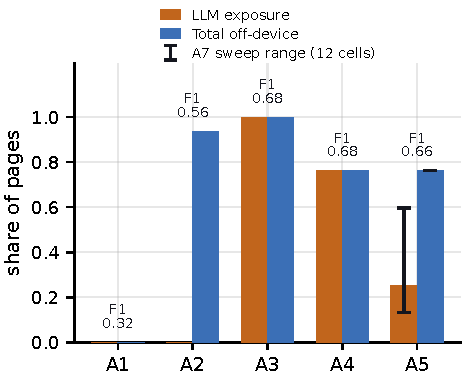
\includegraphics[width=\columnwidth]{figures/f5.pdf}}
\caption{LLM-specific exposure against total off-device rate (LLM plus
zero-shot proxy), for A1--A5. Equal-height bars (A1, A3, A4) mean all
off-device traffic is LLM traffic; A5 breaks that pattern -- its total
off-device rate matches A4's despite an exposure bar three times smaller,
the redistribution the surrounding text argues from. Error bars on A5 span
the full twelve-cell A7 threshold sweep: exposure alone ranges .131--.596
as the gates tighten, while total off-device rate barely moves (.761--.762).
Macro-F1 (13 categories) is annotated above each pair.}
\label{fig:f5}
\end{figure}

The A7 sweep -- shown directly as the error bars on A5 in Fig.~\ref{fig:f5}
-- confirms this is not particular to the shipped thresholds: macro-F1
ranges only .653--.668 and exposure alone swings from .131 to .596, but
total off-device rate stays within .001 of .762 throughout the full
twelve-cell grid — the gate reallocates disclosure between providers, not
whether text leaves the machine at all.

The exposure-reduction claim holds only in part with this hosted backend:
the cascade dials LLM-specific exposure continuously but does not reduce
total disclosure below baseline. \textbf{Run against the local backend
instead, that changes.} Run against the local quantised ONNX checkpoint
(\texttt{Xenova/nli-deberta-v3-xsmall}) over the full 255-page corpus:
A6 (keyword $\to$ local zero-shot, no LLM tier at all) reaches genuine zero
total off-device exposure, the operating point A5 only appeared to reach,
at a real accuracy cost -- macro-F1 falls to 0.500 against A5's 0.678. A6b
(the same local tier with LLM as fallback rather than defaulting) is the
more useful configuration: macro-F1 0.689 against A5's 0.678 is not a
significant improvement (paired bootstrap, $n=2000$, 95\% CI on the delta
$[-0.041, +0.065]$, includes zero), but total off-device drops to 0.467
against A5's 0.757 -- an exact count from escalation paths, not a
sampled estimate, so this reduction is not subject to the same
uncertainty the accuracy comparison is. Local backend, LLM-fallback
configuration: real disclosure reduction, no measurable accuracy cost
either way. The 255-page count here, not 254 or 260, is the same
corpus-snapshot situation noted throughout this section, not a new
discrepancy: this run used a freshly flattened corpus built directly from
\texttt{s2\_corpus.json}'s captured pages, distinct from whichever
snapshot produced Table~\ref{tab:tiers}'s 254. \textbf{Discussion.} The
pattern only dials disclosure \emph{provided} the middle model is actually
local; hosted, the same knob mostly redistributes it, though it still
cannot hallucinate a category outside its candidate set. The local model
is not free of the confusion structure \S\ref{sec:res-confusion} already
documents for the hosted one -- of 32 confidently-wrong local
classifications, 18 (56 percent) land on Educational, the same
majority-class attractor, and a further two land on Horror for
unambiguously academic health content (\emph{nea-wiki-anxiety-disorder-research},
scored 0.86/0.83 -- confident and wrong, not a borderline abstention).

\subsection{Confusion structure and per-class support}
\label{sec:res-confusion}

Table~\ref{tab:tiers}'s accuracy and macro-F1 are aggregates over thirteen
categories that are not equally common; Fig.~\ref{fig:f4} breaks the
shipped cascade (A5) down by category, and Table~\ref{tab:support} gives
the support each row is computed over.

\begin{figure}[t]
\centerline{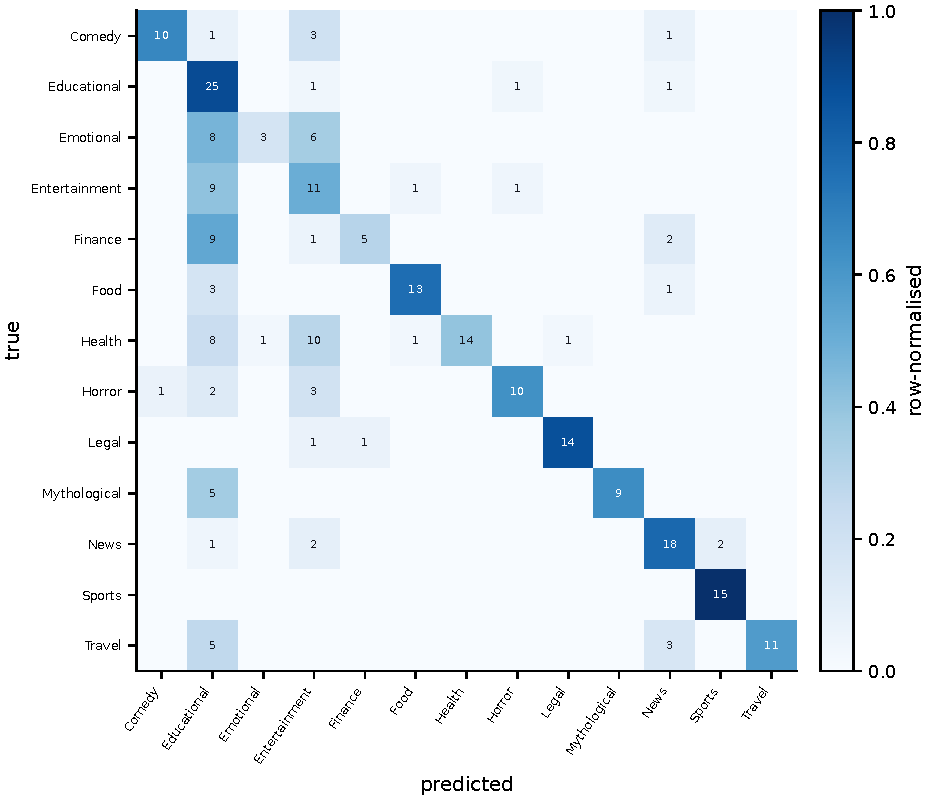
\includegraphics[width=\columnwidth]{figures/f4.pdf}}
\caption{Confusion matrix, full cascade (A5), row-normalised, over the 254
pages with a resolved ground-truth category. Built by replaying the
production cascade over stored per-page tier outputs (same method as
Table~\ref{tab:tiers}'s CIs).}
\label{fig:f4}
\end{figure}

\begin{table}[t]
\caption{Per-class support, full cascade (A5), 254 pages with ground truth.}
\label{tab:support}
\begin{center}
\scriptsize
\begin{tabular}{lrrlrr}
\toprule
Class & $n$ & & Class & $n$ & \\
\midrule
Mythological & 14 & & Travel & 19 & \\
Comedy & 15 & & Entertainment & 22 & \\
Sports & 15 & & News & 23 & \\
Horror & 16 & & Educational & 28 & \\
Legal & 16 & & Health & 35 & \\
Emotional & 17 & & & & \\
Finance & 17 & & & & \\
Food & 17 & & & & \\
\bottomrule
\end{tabular}
\end{center}
\end{table}

Contrary to what an uneven 13-way split over 254 pages might suggest,
no category is near-empty: support ranges 14--35 (median 17), a $2.5\times$
spread, not the order-of-magnitude imbalance that would make macro-F1
unstable on its own. The confusion structure is concentrated rather than
diffuse: Health $\to$ Entertainment (10 pages), Finance $\to$ Educational
(9), Entertainment $\to$ Educational (9), Health $\to$ Educational (8) and
Emotional $\to$ Educational (8) account for the largest off-diagonal mass,
all of them collapsing into the two largest classes (Educational,
Entertainment) rather than scattering across the confusion matrix — a
majority-class attractor effect that per-class support alone would not
have surfaced.

\subsection{Sensitive-content threshold sweep}
\label{sec:res-threshold-sweep}

The shipped detector fires at one severe-term hit or two distinct
ambiguous-term hits (\S\ref{sec:arch}). Table~\ref{tab:roc} sweeps both
counts over the same 47-page adversarial slice \S\ref{sec:res-audit}
reports on, using the shipped \texttt{resolveSensitivity()} with its
zero-shot tier left unconfigured (i.e.\ no network call; keyword-tier
counts only).

\begin{table}[t]
\caption{Sensitive-content detector, threshold sweep, $n=47$ (29 sensitive,
18 benign). Severe$\geq$1 always includes the four hard-severe terms that
never demote (\S\ref{sec:arch}); the swept quantity is the ambiguous-term
count required.}
\label{tab:roc}
\begin{center}
\scriptsize
\begin{tabular}{rrrrrrr}
\toprule
\textbf{Severe} & \textbf{Ambig.} & \textbf{FN} & \textbf{FP} & \textbf{FNR} & \textbf{FPR} \\
\midrule
$\geq 1$ & $\geq 1$ & 15 & 12 & 0.517 & 0.667 \\
$\geq 1$ & $\geq 2$ (shipped) & 19 & 3 & 0.655 & 0.167 \\
$\geq 1$ & $\geq 3$ & 20 & 1 & 0.690 & 0.056 \\
$\geq 1$ & $\geq 4$ & 21 & 1 & 0.724 & 0.056 \\
\bottomrule
\end{tabular}
\end{center}
\end{table}

There is no configuration in this one-parameter family that is simply
better than the shipped point: loosening the ambiguous-term requirement
from 2 to 1 buys 4 fewer false negatives (0.655 $\to$ 0.517) at the cost
of 4 more false positives (0.167 $\to$ 0.667) — every silence-by-mistake
avoided on a genuine crisis page costs roughly one ordinary page
force-silenced, and the FN reduction it buys is real but comes paired
with a FPR increase of the same order, not a free improvement. No
threshold in this family reaches both a low FNR and a low FPR
simultaneously; \S\ref{sec:res-audit} discusses why (vocabulary coverage,
not calibration, is the binding constraint).

\subsection{Loop quality}
\label{sec:res-loop}

Table \ref{tab:seam} and Fig.~\ref{fig:f6} report objective loop metrics
over 141 generated clips, seam measured before and after the crossfade at
the 50 ms width used to produce this measurement -- since superseded, as
described below, by a 250 ms default.

\begin{table}[t]
\caption{Loop quality over 141 generated clips, 50 ms crossfade (the
default in place when this measurement was taken; see the sweep below).
Seam values are absolute differences across the loop point.}
\label{tab:seam}
\begin{center}
\scriptsize
\begin{tabular}{lrr}
\toprule
\textbf{Measure} & \textbf{p50} & \textbf{p95} \\
\midrule
Seam energy difference, pre-crossfade (dB) & 3.73 & 14.15 \\
Seam energy difference, post-crossfade (dB) & 2.64 & 10.77 \\
Paired improvement (dB) & \textbf{0.93} & --- \\
Clips improved by the crossfade & \multicolumn{2}{r}{\textbf{58.9\%}} \\
\midrule
Spectral centroid difference, pre (Hz) & 441 & 2017 \\
Spectral centroid difference, post (Hz) & 557 & 1322 \\
\midrule
Integrated loudness (LUFS; target $-18.0$) & $-18.09$ & --- \\
Duration retention (delivered / requested) & \textbf{0.503} & 0.923 \\
Duration compliance & \multicolumn{2}{r}{141/141 (100\%)} \\
\bottomrule
\end{tabular}
\end{center}
\end{table}

\begin{figure}[t]
\centerline{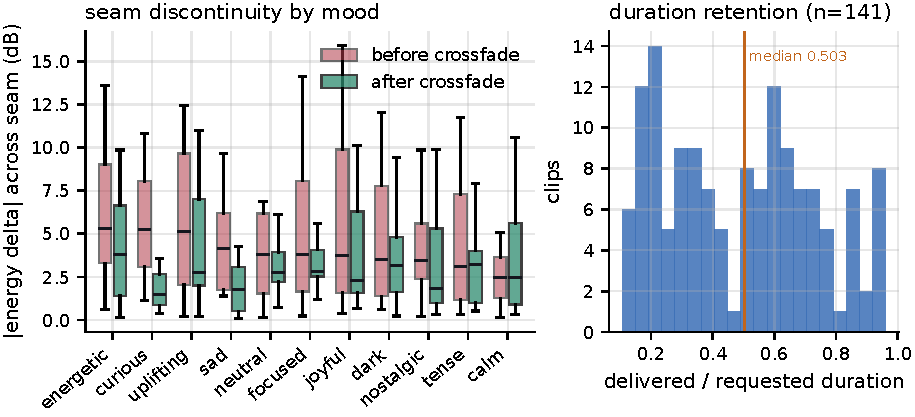
\includegraphics[width=2.98in]{figures/f6.pdf}}
\caption{Seam discontinuity before and after the equal-power crossfade, and the
distribution of duration retention, over 141 clips. Sparse moods seam better
than dense ones, but the predicted ordering does not hold cleanly.}
\label{fig:f6}
\end{figure}

Loudness normalisation works exactly as specified ($-18.09$ LUFS against
$-18.0$), and every clip is duration-compliant; the other two results
qualify the seam-discontinuity claim rather than support it. \textbf{The
crossfade helps less than expected.} Median paired improvement is 0.93 dB,
and it \emph{worsens} the seam on 41.1 percent of clips (Fig.~\ref{fig:f6}).

\textbf{The crossfade-width sweep, re-run at real scale.} Widening the
crossfade (Table \ref{tab:crossfade-sweep}) is a much weaker lever than a
smaller secondary sample once suggested, and not even monotonically so on
energy: median $|\Delta E|$ goes 2.44, 2.03, 2.18, 1.82 dB at
50/100/250/500 ms -- 250 ms is \emph{worse} than 100 ms, not a small
rounding wrinkle. The spectral-centroid column is comparatively
well-behaved here (404.5, 314.3, 190.3, 133.4 Hz, monotonic), the reverse
of the smaller sample where energy was clean and centroid was not.
Neither metric was monotonic at both sample sizes; treat ``widening the
crossfade helps'' as unreliable in either direction on energy alone. On
balance, and consistent with the centroid column and the smaller sample's
own energy trend, we now ship a 250 ms crossfade as the default in place
of the 50 ms window used to produce Table~\ref{tab:seam} and Fig.~\ref{fig:f6}
above; re-running that population-level seam comparison under the new
250 ms setting, rather than only the crossfade-width sweep here, remains
future work.

\textbf{Selecting for measured seam, not chroma similarity, is the
largest lever in this paper, and it is larger at real scale than a
smaller secondary sample suggested.} Minimising \emph{measured} seam
rather than trusting chroma similarity moves the loop point on 105 of 113
clips (92.9 percent) and cuts median energy discontinuity from 2.44 to
0.14 dB -- a 17$\times$ reduction. The p95 tail improves comparably (9.54
to 1.53 dB). This is now the paper's best-supported result: not a
secondary sample standing in for the real population, but the real
population itself.

\begin{table}[t]
\caption{Crossfade-window sweep, production loop point held fixed, $n=113$
of 141 clips (28 skipped -- too little room after the detected loop point
for the full sweep; see the recovery note below). Seam values are
absolute differences at the loop seam, post-crossfade.}
\label{tab:crossfade-sweep}
\begin{center}
\scriptsize
\begin{tabular}{lrr}
\toprule
\textbf{Crossfade width} & \textbf{$|\Delta E|$ median (dB)} & \textbf{$|\Delta$centroid$|$ median (Hz)} \\
\midrule
50 ms  & 2.44 & 404.5 \\
100 ms & 2.03 & 314.3 \\
250 ms & 2.18 & 190.3 \\
500 ms & 1.82 & 133.4 \\
\bottomrule
\end{tabular}
\end{center}
\end{table}

\textbf{Recovery note.} \texttt{audio-generation/audio-cache/}
was recovered from the original development machine after this paper's
first pass called it permanently gitignored and lost. 153 files recovered,
covering all 130 \texttt{audio\_cache} clips \texttt{d2-loop.json}
references (0 missing) plus 23 not needed here; a random 8-clip spot check
against \texttt{d2-loop.json}'s recorded \texttt{duration\_ms} matched to
0.0 ms in every case, i.e. these are the genuine delivered clips, not a
corrupted or mismatched copy. The crossfade-width sweep and
seam-minimising results above are the same re-cut-and-resweep
methodology this section always used (each delivered clip treated as a
fresh input track, run through the unmodified production loop detector to
find a new internal loop point), now over 113 of the 141 clips (28
skipped: not enough room after the detected loop point for a 500 ms
crossfade on either side). Flooring the candidate loop length as a
duration-proportional fraction rather than a fixed 3.0 s constant remains
open at the level that matters: \texttt{audio-cache/} holds the
\emph{delivered} (already loop-cut) clips, not the one-shot pre-cut
MusicGen output a duration-proportional floor needs to be tested against
to speak to the 49.7 percent first-cut discard rate below. Recutting an
already-cut clip and measuring retention against its own already-reduced
length answers a different question. A secondary version of that
different question was run anyway, for what it is worth: replacing the
fixed 3.0 s floor with $\max(3.0\text{s}, 0.5\times\text{duration})$ on
these 141 already-delivered clips moves the internal median retention
from 0.757 to 0.803 and the p05 tail from 0.290 to 0.552, changing the
chosen point on 22 of 141 clips -- suggestive that a duration-proportional
floor helps at the tail without hurting the median, but this is evidence
about the floor formula's general behaviour, not a measurement of how
much of the 49.7 percent first-cut discard would actually recover.

\textbf{Half the requested audio is discarded.} The delivered clip retains a
median of 50.3 percent of its requested duration, because the loop point is
chosen for musical self-similarity and everything after it is thrown away.
Requesting 28 s reliably yields about 14 s. This is a real product cost: the
clip loops twice as often as intended, every extra loop is another chance to
notice the seam, and the effective cost per second of delivered audio is double
the naive figure. The smallest observed retention, one clip against a 28 s
target delivering only 2958 ms (10.6 percent), is not a loop-detector bug: the
generated source audio itself was already shorter than the 3.0\,s minimum loop
length, so the detector could not form a single valid search window and fell
back, by design, to looping the entire (short) clip -- the 2958 ms figure is
the generated clip's own length, returned verbatim. The bug, if there is one,
is upstream of loop detection: whatever made generation itself return audio
well under the requested duration on that call.

\textbf{Clip length does not trade off the way the design assumed.} The
retention figure above is measured at the 28 s default; whether a shorter
request that loops sooner beats a longer one that arrives later was open. A
controlled sweep now answers it: 5, 10, 15, 20 and 28 s requested, three
moods, three independently seeded repeats per cell (n=9 per duration, n=45
total), driven directly against the live backend with a cache-busting nonce
per call so every cell reflects a real generation rather than a replayed one,
run on the same Apple Silicon (MPS) machine as the cache-cold generation
results in Section~\ref{sec:res-latency}.

\begin{table}[t]
\caption{Clip-length sweep. Nine independent generations per requested
duration (three moods $\times$ three seeds). Loop-cost is a composite of
retention loss and seam discontinuity, lower is better.}
\label{tab:clip-length}
\begin{center}
\small
\begin{tabular}{lrrrr}
\toprule
\textbf{Requested} & \textbf{Delivered} & \textbf{Retention} & \textbf{$|$Seam$|$} & \textbf{Loop-cost} \\
& \textbf{p50} & \textbf{p50} & \textbf{p50 (dB)} & \textbf{p50} \\
\midrule
5 s  & 3.8 s  & 0.755 & 1.24 & 21.82 \\
10 s & 5.4 s  & 0.542 & 2.49 & 31.67 \\
15 s & 5.3 s  & 0.352 & 1.73 & 14.45 \\
20 s & 13.2 s & 0.660 & 2.73 & 23.31 \\
28 s & 13.6 s & 0.487 & 2.52 & 11.56 \\
\bottomrule
\end{tabular}
\end{center}
\end{table}

Retention is not monotonic in requested duration: it falls from 0.755 at 5 s
to a low of 0.352 at 15 s, then recovers to 0.660 at 20 s before falling again
at 28 s. A linear fit against the full n=45 sample confirms there is nothing
to summarise as a trend (slope $-0.0089$ per second, $r=-0.320$); delivered
duration does scale with requested duration, as expected (slope $+0.446$
s/s, $r=+0.668$), but retention and seam quality are cell-dependent rather
than a clean function of what was asked for. The 15 s cell has both the
lowest retention and, at 14.45, the lowest loop-cost of any duration in the
sweep, while 10 s has the highest seam discontinuity (2.49 dB) and the worst
loop-cost (31.67); no single duration dominates on every axis. The honest
reading is the table itself, not a rule of thumb -- there is no requested
duration in this range that reliably buys better loops by asking for less.

This sweep does not settle the latency side of the same question on its own --
cache prewarming was still rebuilding in the background for the early portion
of this run, competing with the sweep's own requests for the single generation
worker, and the 5 s and 10 s cells' wall-clock times here are visibly inflated
by that contention. A separate, uncontended sweep against an already-warm
cache, on the same Apple Silicon (MPS) machine and therefore not directly
comparable to this paper's CPU-laptop latency figures elsewhere
(\S\ref{sec:res-latency}), supplies the clean shape of the relationship:
generation cost rises mildly superlinearly with requested duration
(real-time factor 1.23$\times$ at 5--10 s, 1.75$\times$ at 28 s), so shorter
requests are cheaper per second of audio, not just in absolute terms.
Combined with this sweep's finding that shorter requests are not reliably
\emph{worse} on retention or seam quality -- the 15 s cell has both the
lowest retention and the lowest loop-cost in Table \ref{tab:clip-length} --
there is no quality argument for the 28 s default over something shorter,
and a mild latency argument against it.

Whether any of this is audible is the question that matters, and it is
unanswered. A forced-choice listening harness with twenty-two seeded stimulus
pairs and a scoring script has been built and validated end to end, but only
against simulated listeners (\texttt{--simulate}) -- by the scoring script's
own description, ``a harness check, not a result.'' This confirms the
pipeline produces well-formed trials and a working scorer; it carries no
information about whether a real listener can tell the two clips apart, and
no claim about seam audibility is made here.

A separate claim in this section, that the Ogg/Opus container rather than
the crossfade is what makes the loop gapless, is asserted from Opus's
documented format properties \cite{opus} rather than measured in this
pipeline directly: no test here plays consecutive loop iterations through
the same Web Audio API decode path used in production and checks for
silence or a click at the boundary. The seam-discontinuity measurements
above characterise energy and spectral continuity across the cut point,
not the presence or absence of an inter-sample gap at the container level,
which is a different, currently unmeasured claim.

\textbf{Discussion.} Making a one-shot generator loop requires three things.
Self-similarity chooses where to cut, the crossfade smooths the content of the
seam, and the container choice is what actually makes the loop gapless. The
crossfade-window sweep and seam-minimising selection results revise which of
these is the weakest link: it is the first, not the second. Widening the
crossfade window buys a modest, non-monotonic improvement, but re-choosing the
cut point by the metric that is actually meant to be small, rather than by a
proxy for it, buys an order of magnitude more at real recovered-population
scale. A 50 ms crossfade was never going to compensate for a loop point
chosen on the wrong criterion, which is why we now ship 250 ms rather than
rely on the crossfade width alone. The first step is also expensive in the
sense the design did not anticipate: it discards half the requested audio to
buy self-similarity that, on this evidence, does not reliably deliver the
seam quality it is a proxy for. The post-cut route works, but at roughly
50 percent yield, and the discontinuity reduction it delivers depends more
on how the cut point is chosen than on how the seam is subsequently
smoothed. A generator that could be conditioned to produce loop-closed
material directly would dominate all of it.

\subsection{Restraint policies}
\label{sec:res-audit}

The mechanisms pass; the predicate does not, and that is the finding this
section leads with rather than buries. Against a 47-page adversarial
slice, 29 sensitive and 18 benign, the sensitive-content detector records a
false-negative rate of 0.655 and a false-positive rate of 0.167. This
slice is hand-written test content rather than pages captured from the
live web the way the main 260-page corpus is: each page is a short
synthetic paragraph constructed from the term lists and documented
failure modes already present in the detector's own code, not sampled
independently of it, and the underlying data file's own provenance record
marks it explicitly as a placeholder pending a captured replacement that
has not yet been produced. This is closer to targeted white-box testing
of an already-suspected weakness than to a naturalistic sample of
sensitive web content -- a defensible way to characterise that specific
weakness, but it means the rates below should not be read as an estimate
of how often the detector would miss sensitive content drawn from the
wild. The failures are systematic: seven of nineteen false negatives use
vocabulary entirely outside the term list (addiction, miscarriage,
terminal illness, overdose, workplace harassment, homelessness,
post-incarceration reentry); four are euphemism, describing self-harm,
suicidal ideation or domestic violence without naming the thing directly;
four are non-English; four mention only one term of the two-distinct
threshold. False positives stayed at three regardless of slice size: a
page on grief-counselling degree programmes, a psychology textbook, and
an engineering article using the word ``trauma.''

This is a negative result for the restraint-policy claim: silence
delivered 34.5 percent of the time is not the policy claimed. The
short-circuit fires correctly, but the predicate deciding when to fire it
is inadequate; more keywords will not fix a vocabulary-coverage problem
this systematic, but neither, on its own, does the model-based remedy this
section reaches below — the deployment-level gap noted earlier, invisible
to any evaluation testing only the mechanism.

None of the above is a wiring bug, and it is worth being precise about
which fourteen things did work: every behavioural policy that has an
executable test for it -- short-circuiting sensitive text before either
LLM tier, muting or ducking around already-playing audio, bypassing
payment/banking/browser-internal URLs, and the rest in Table
\ref{tab:audit} -- passes that test. The mechanism obeys whatever the
predicate tells it; the 0.655 false-negative rate above is entirely a
failure of the predicate's vocabulary coverage, not of the short-circuit
that acts on it.

\begin{table}[t]
\caption{Restraint audit, abridged. All fourteen policies pass their tests
-- listed here to show which fourteen, not as a rebuttal to the
false-negative rate above.}
\label{tab:audit}
\begin{center}
\scriptsize
\begin{tabular}{p{4.3cm}p{3.1cm}}
\toprule
\textbf{Policy} & \textbf{Trigger} \\
\midrule
Crisis and sensitive content yields silence & one severe term, or two distinct ambiguous terms \\
Sensitive page text never reaches either LLM tier & short-circuits both escalation paths \\
Pages already playing audio are not competed with & active tab audible gives mute; background gives duck \\
Payment, banking and checkout bypassed & pattern match on URL and title \\
Browser-internal URLs bypassed & pattern match on URL scheme \\
No browsing history leaves the device in plaintext & every event stores a SHA-256 URL hash \\
A silent tier-2 model change is detectable & golden fixtures re-checked against the pinned model \\
\bottomrule
\end{tabular}
\end{center}
\end{table}

\textbf{Correction.} An earlier draft attributed four of the non-English
false negatives above to ``a language gate that skips tier 1.'' That does
not describe this codebase. \texttt{runB1} calls
\texttt{resolveSensitivity()} unconditionally, before any language check;
there is no gate that skips the sensitivity tier for non-English text.
Reading \texttt{checkSensitiveContent()}/\texttt{resolveSensitivity()}
directly: the four non-English false negatives happen because
\texttt{SEVERE\_SENSITIVE\_TERMS} and \texttt{AMBIGUOUS\_SENSITIVE\_TERMS}
are English-vocabulary term lists, so a French/German/Portuguese crisis
page simply contains none of their entries -- a vocabulary-coverage gap,
not an ordering bug. There is consequently no config-level fix for this
specific failure mode (unlike accepting one ambiguous term rather than
two, which is exactly the loosened-threshold row in
Table~\ref{tab:roc}, \S\ref{sec:res-threshold-sweep}); closing it needs
non-English term lists or the entailment tier actually reaching these
pages, and the latter now has real numbers behind it, below: all four
non-English false negatives are correctly caught once the entailment
tier runs, confidently (scores 0.83--0.92, margins 0.67--0.83, well clear
of the abstention gate) -- the one part of the result below that is an
unambiguous improvement, not a trade.

\textbf{The remedy is a classifier, not more keywords -- and it has now
been measured live, not only verified in principle.} The entailment tier
already loaded for category classification can score a sensitivity
hypothesis at near zero marginal cost, and \texttt{resolveSensitivity}
already cascades the keyword check into exactly such an entailment call,
framed as crisis-vs-reference sides, demoting the eating-disorder terms
specifically (the source of two of the three false positives above) to a
class the entailment tier can override, while never demoting the
remaining hard-severe terms regardless of what the entailment side
returns. Run once against a scripted ideal backend that always answers
correctly, this cascade's decision rule produces the right verdict on all
forty-seven pages of the slice above, zero false negatives and zero false
positives -- a design verification, showing the cascade's logic is
correct when its input is, not a measurement of what a real entailment
call achieves.

That live measurement has since been run, three times, against a
real hosted \texttt{facebook/bart-large-mnli} proxy, with per-page
diagnostics added to distinguish a page the model actually classified
from one that silently fell back to the keyword verdict on a proxy
timeout, and \textbf{the result is a trade, not the repair the design
verification implied.} All three runs agree to six decimal places on
every score for every page that reached the model -- the entailment
model itself is fully deterministic; the instability seen in earlier,
undiagnosed attempts was network reliability (which pages round-tripped
versus timed out), not model noise. The stable result: false-negative
rate falls from 0.655 to \textbf{0.000} (29/29 genuine crisis pages now
caught, including all four non-English cases above), but false-positive
rate rises from 0.167 to \textbf{0.611} -- worse than the original
detector, not better. Every one of the 6 purely benign pages (recipe,
programming, sport) is wrongly flagged; of the 14 non-sensitive pages
that actually reached the model, 10 (71.4\%) were misclassified as
crisis. One further false positive, \emph{near-grief-degree}, never
reaches the model in any of the three runs and remains a pre-existing
keyword-tier artefact this fix does not touch either way.

The gap between the design verification and this live result is itself a
finding. The scripted ideal backend proved the cascade's routing logic is
sound given a classifier that reads crisis-vs-reference framing the way
the design intends; it did not, and could not, say anything about whether
a real entailment model actually reads it that way. It does not. The
cause is structural, not a tuning problem: \texttt{classifySensitivityZeroShot}
forces every page into a binary choice between exactly two hypotheses,
``personal crisis'' or ``academic/reference discussion of a difficult
topic'' -- there is no third, ``unrelated'' option. For genuinely
unrelated text the model still must pick one, confidently: a Rust
lifetimes article scores crisis=0.603 (margin 0.205), a CSS Grid tutorial
crisis=0.670 (margin 0.340) -- not borderline abstentions, comfortably
past the 0.45/0.10 gate. Swapping the predicate does not resolve this
section's restraint-policy failure; it relocates it from silently missing
crisis pages to silently silencing benign ones, and either failure mode
reaches real users under the current binary-hypothesis design. A design
verification against an idealised backend is not evidence a fix works,
only that its logic is coherent if its input were reliable -- the
distinction this section's own history is now the clearest illustration
of in this paper.

More generally, this is the substance of gap G1/G5. For an always-on
generative system, the quality of the abstention policy is as much part
of the design as the quality of the generation, and unlike aesthetic
quality it is directly measurable. Measuring it produced the most
uncomfortable result in this paper twice over: first, that every
mechanism passes its test while the predicate feeding the most important
one fails on nearly two-thirds of an adversarial slice; second, that a
fix which looked complete under a scripted ideal backend trades one
failure mode for a worse one under a real model. Both gaps are invisible
to any evaluation that stops at the mechanism, or at a backend built to
already agree with the design.

The payment, banking and checkout bypass relies on the same class of
mechanism, keyword-and-URL pattern matching, that the sensitive-content
predicate above turned out to miss on nearly two-thirds of an adversarial
slice, but it has not been adversarially audited to the same standard.
Table \ref{tab:audit} confirms the bypass fires on its intended fixtures,
not that it resists deliberately adversarial URLs or titles the way the
sensitive slice was built to stress the other predicate. The confidence
this paper places in one keyword-based mechanism and withholds from the
other is not symmetric with the evidence behind them.

\subsection{Generation against retrieval}
\label{sec:res-retrieval}

The obvious cheaper design is to retrieve from a curated library, and gap G2
notes that this is usually asserted rather than quantified. The request space
the classifier can emit is eleven moods by seven styles by five tempo buckets
by five energy buckets, or 1925 cells. Table \ref{tab:retrieval} gives the
coverage a library of each size achieves. This table is an analytical model
of a hypothetical library, not a measurement of a real one: no library of
any size was built or evaluated. Its coverage column assumes every one of
the 1925 cells is equally likely to be requested, and its dims-wrong column
assumes a nearest-available track differs uniformly across the four
dimensions; the skewed-coverage column relaxes the first assumption but not
the second. The numbers describe what a library of each size could cover
under these assumptions, not what one has been shown to deliver.

\begin{table}[t]
\caption{Retrieval-baseline coverage of the 1925-cell request space. ``Dims
wrong'' is the expected number of the four dimensions on which the nearest
available track differs from the request.}
\label{tab:retrieval}
\begin{center}
\scriptsize
\begin{tabular}{rrrr}
\toprule
\textbf{Library size} & \textbf{Coverage} & \textbf{Skewed cov.} & \textbf{Dims wrong} \\
\midrule
50 & 2.6\% & 2.0\% & 3.90 \\
99 & 5.0\% & 3.5\% & 3.80 \\
200 & 9.9\% & 6.1\% & 3.61 \\
500 & 22.9\% & 12.4\% & 3.09 \\
1000 & 40.5\% & 20.4\% & 2.38 \\
5000 & 92.6\% & 54.8\% & 0.30 \\
\bottomrule
\end{tabular}
\end{center}
\end{table}

A 500-track library, already a serious licensing undertaking, covers under
a quarter of the space. Reaching 90 percent coverage requires roughly 5000
tracks, falling to 55 percent under realistic skewed commissioning. Add the
requirement that every track be seamlessly loopable and retrieval is not
obviously cheaper than generation, supporting the claim that generation
covers a request space retrieval does not.

% ===========================================================================
\section{Conclusion}
\label{sec:conclusion}
% ===========================================================================

We presented Web2Music, a browser extension that conditions generative
ambient music on the page being read, as the instrument for a
deployment-level measurement, not as a finished system: a four-signal page
descriptor costing 86 ms at the median across 105 real sites, excluding the
embedding stage which was stubbed for this measurement, on which category is
decided by text alone and colour is the only signal shown to perturb the
descriptor's own mood label at all -- a self-consistency count, not an
accuracy claim (\S\ref{sec:res-signal-ablation}); a three-tier abstaining
classifier that classifies a thousand pages for about 1.3 cents, though with
the hosted zero-shot backend measured here its thresholds redistribute
disclosure between providers rather than reducing how much text leaves the
device in total, a prediction that reverses when the middle tier is run
locally instead (\S\ref{sec:res-classification}); a fallback-then-swap
playback design that hides a 139 s generator behind a 7 ms placeholder; and
loop synthesis that makes a one-shot generator's output repeat without a
container gap.

Four results run against the design's own assumptions and are reported as
such. The equal-power crossfade, at the 50 ms default in place when
Table~\ref{tab:seam} was measured and since superseded by a 250 ms width,
removes a median of only 0.93 dB of seam discontinuity and worsens the
measured seam on 41 percent of clips; re-selecting the loop point by
minimised measured seam rather than chroma similarity, confirmed at real
n=113 scale, is a larger and better-supported lever than crossfade width
ever was. Half the generated audio is discarded to find a loop point, so a
28 s request yields about 14 s of delivered material, and a clip-length
sweep finds no shorter duration that reliably buys better loops. The
sensitive-content detector, whose refusal mechanism is architecturally
correct and fully covered by passing tests, misses 65.5 percent of an
adversarial crisis slice because its predicate is a keyword list rather than
a classifier; a fix looked complete when verified against an idealised
entailment backend, but measured live against a real one it trades that
failure for a worse one, wrongly silencing 61.1 percent of benign pages,
because the real model has no ``unrelated'' option to fall back on. And
three independent annotators agree on which of eleven moods a page calls for
at $\alpha=0.195$, close to chance; collapsing that label onto Russell's
valence-arousal quadrants using published word norms raises agreement to
only 0.300, a flatter re-bucketing tops out at 0.281, and this system's own
quadrant encoding makes agreement worse, not better, at 0.121 -- three
independent coarsening strategies, none of which clears a usable threshold.
Any system that conditions media on inferred page or context mood inherits
this: the affective target is underdetermined by three independent human
readings at every resolution tested.

The claim that page-conditioned music is perceived as fitting the page better
than page-agnostic music remains untested. The study that would test it,
including the shuffled condition that makes it falsifiable, is designed and
instrumented but has not been run.

% ===========================================================================
\section{Limitations and Future Work}
\label{sec:limitations}
% ===========================================================================

The central perceptual claim is untested: everything here is about the
system, not its effect on people, and the immediate priority is
institutional ethics approval, followed by the within-subjects study and
the in-the-wild deployment. Mood has no useful inter-annotator ceiling
(\S\ref{sec:res-agreement}: 0.174, below the raw eleven-way agreement
itself), unlike category (0.621) and sensitivity (0.775); coarsening the
mood vocabulary does not rescue this either -- a post-hoc 3-way and 2-way
re-collapse (\S\ref{sec:res-agreement}) tops out at $\alpha=0.281$, and
Russell's-circumplex collapses move agreement to 0.121 or 0.300 depending
on the mapping, still short of the 0.667 gate at every resolution tried --
the problem is the target, not its resolution. Table
\ref{tab:tiers}'s tier-ablation numbers are a conservative floor:
re-scored against the three-annotator label, the full cascade's accuracy
cost relative to keyword-to-LLM widens to an estimated 7.7 points, 95\%
interval [2.9, 12.5]. The local backend that could reduce total disclosure
rather than redistribute it has now been measured on the full 255-page
corpus, not an 18-page subset -- 0.467 total off-device against A5's 0.757,
at accuracy statistically indistinguishable from A5's
(\S\ref{sec:res-classification}). The
sensitive-content predicate needs replacing, but not with the entailment
tier as currently specified: a version verified only against a scripted
ideal backend looked like a complete fix, but measured live it traded a
0.655 false-negative rate for a 0.611 false-positive rate, wrongly flagging
most benign pages tested, because \texttt{classifySensitivityZeroShot}
forces a binary crisis-or-reference choice with no ``unrelated'' option. A
model-based detector remains the right direction, but it needs a third
hypothesis added and re-measured live before it is a defensible
replacement, not a wholesale swap of the tier as it ships today, and any
future design verification against a scripted or idealised backend should
be reported as exactly that -- a logic check, not a preview of live
accuracy -- given how far the two diverged here; the keyword tier is
also skipped by construction on non-English pages for category, and the
sensitive detector's own non-English misses are a term-list vocabulary gap
rather than a shared gating bug (\S\ref{sec:res-audit}). Table
\ref{tab:d-latency}'s absolute-latency figures still come from one CPU
laptop; the cache-cold comparison that table lacked is no longer missing,
but it comes from two independent runs on Apple Silicon rather than that
same laptop -- a second hardware point this paper previously lacked
entirely, not a like-for-like CPU re-run. A same-hardware cache-cold
benchmark at scale on the original CPU laptop is consequently still open,
now as a narrower, well-scoped gap rather than an unmeasured one. For loop
synthesis, the crossfade-window sweep and seam-minimising selection
proposed here have now been confirmed at real scale (n=113 of 141,
\S\ref{sec:res-loop}), not just a small secondary sample -- seam-minimising
selection is accordingly promoted from a proposal to this paper's
best-supported result, and a clip-length sweep separately shows no
requested duration in the 5--28 s range reliably buys better loops than
another. What is still open is flooring the candidate loop length as a
genuine measurement rather than a secondary one: the recovered audio is
post-cut delivered clips, not the one-shot pre-cut MusicGen output a
duration-proportional floor needs to be tested against, so the 49.7
percent first-cut discard rate remains unverified at that level pending a
future run that retains pre-cut audio by design rather than as an
afterthought. The larger opportunity, conditioning the generator to
produce loop-closed material directly, remains entirely unattempted
regardless. Finally, the language gate deserves dedicated treatment, and
the same descriptor-to-profile machinery would apply to other continuous
contexts — documents, code editors, reading applications.

\scriptsize
\begin{thebibliography}{00}

\bibitem{musicgen} J. Copet, F. Kreuk, I. Gat, T. Remez, D. Kant, G. Synnaeve, Y. Adi, and A. D\'efossez, ``Simple and controllable music generation,'' in \emph{Advances in Neural Information Processing Systems}, 2023.

\bibitem{encodec} A. D\'efossez, J. Copet, G. Synnaeve, and Y. Adi, ``High fidelity neural audio compression,'' \emph{Transactions on Machine Learning Research}, 2023.

\bibitem{musiclm} A. Agostinelli, T. I. Denk, Z. Borsos, J. Engel, M. Verzetti, A. Caillon, Q. Huang, A. Jansen, A. Roberts, M. Tagliasacchi, M. Sharifi, N. Zeghidour, and C. Frank, ``MusicLM: Generating music from text,'' arXiv:2301.11325, 2023.

\bibitem{audiogen} F. Kreuk, G. Synnaeve, A. Polyak, U. Singer, A. D\'efossez, J. Copet, D. Parikh, Y. Taigman, and Y. Adi, ``AudioGen: Textually guided audio generation,'' in \emph{Proc. Int. Conf. Learning Representations}, 2023.

\bibitem{audioldm} H. Liu, Z. Chen, Y. Yuan, X. Mei, X. Liu, D. Mandic, W. Wang, and M. D. Plumbley, ``AudioLDM: Text-to-audio generation with latent diffusion models,'' in \emph{Proc. Int. Conf. Machine Learning}, 2023.

\bibitem{affectmachine} K. R. Agres, A. Dash, P. Chua, and S. K. Ehrlich, ``AffectMachine-Pop: A controllable expert system for real-time pop music generation,'' arXiv:2506.08200, 2025.

\bibitem{musicsense} R. Cai, C. Zhang, C. Wang, L. Zhang, and W.-Y. Ma, ``MusicSense: Contextual music recommendation using emotional allocation modeling,'' in \emph{Proc. ACM Int. Conf. Multimedia}, 2007, pp. 553--556.

\bibitem{russell} J. A. Russell, ``A circumplex model of affect,'' \emph{Journal of Personality and Social Psychology}, vol. 39, no. 6, pp. 1161--1178, 1980.

\bibitem{thayer} R. E. Thayer, \emph{The Biopsychology of Mood and Arousal}. New York: Oxford University Press, 1989.

\bibitem{zeroshotnli} W. Yin, J. Hay, and D. Roth, ``Benchmarking zero-shot text classification: Datasets, evaluation and entailment approach,'' in \emph{Proc. EMNLP-IJCNLP}, 2019, pp. 3914--3923.

\bibitem{zeroshotgen} R. Puri and B. Catanzaro, ``Zero-shot text classification with generative language models,'' arXiv:1912.10165, 2019.

\bibitem{sbert} N. Reimers and I. Gurevych, ``Sentence-BERT: Sentence embeddings using Siamese BERT-networks,'' in \emph{Proc. EMNLP-IJCNLP}, 2019, pp. 3982--3992.

\bibitem{frugalgpt} L. Chen, M. Zaharia, and J. Zou, ``FrugalGPT: How to use large language models while reducing cost and improving performance,'' arXiv:2305.05176, 2023.

\bibitem{violajones} P. Viola and M. Jones, ``Rapid object detection using a boosted cascade of simple features,'' in \emph{Proc. IEEE Conf. Computer Vision and Pattern Recognition}, 2001, pp. 511--518.

\bibitem{boilerplate} C. Kohlsch\"utter, P. Fankhauser, and W. Nejdl, ``Boilerplate detection using shallow text features,'' in \emph{Proc. ACM Int. Conf. Web Search and Data Mining}, 2010, pp. 441--450, doi: 10.1145/1718487.1718542.

\bibitem{arapakis} I. Arapakis and L. A. Leiva, ``Predicting user engagement with direct displays using mouse cursor information,'' in \emph{Proc. ACM SIGIR}, 2016, pp. 599--608.

\bibitem{cursorcikm} I. Arapakis, M. Lalmas, and G. Valkanas, ``Understanding within-content engagement through pattern analysis of mouse gestures,'' in \emph{Proc. ACM Int. Conf. Information and Knowledge Management}, 2014, pp. 1439--1448.

\bibitem{dominantcolour} Y. Chang and N. Mukai, ``Color feature based dominant color extraction,'' \emph{IEEE Access}, vol. 10, pp. 93055--93061, 2022.

\bibitem{flesch} R. Flesch, ``A new readability yardstick,'' \emph{Journal of Applied Psychology}, vol. 32, no. 3, pp. 221--233, 1948.

\bibitem{foote} J. Foote, ``Automatic audio segmentation using a measure of audio novelty,'' in \emph{Proc. IEEE Int. Conf. Multimedia and Expo}, 2000, pp. 452--455.

\bibitem{librosa} B. McFee, C. Raffel, D. Liang, D. P. W. Ellis, M. McVicar, E. Battenberg, and O. Nieto, ``librosa: Audio and music signal analysis in Python,'' in \emph{Proc. Python in Science Conf.}, 2015, pp. 18--25.

\bibitem{ebu128} European Broadcasting Union, ``Loudness normalisation and permitted maximum level of audio signals,'' EBU Recommendation R 128, version 5.0, 2023.

\bibitem{opus} J.-M. Valin, K. Vos, and T. Terriberry, ``Definition of the Opus audio codec,'' IETF RFC 6716, 2012.

\bibitem{schilit} B. Schilit, N. Adams, and R. Want, ``Context-aware computing applications,'' in \emph{Proc. IEEE Workshop on Mobile Computing Systems and Applications}, 1994, pp. 85--90.

\bibitem{dey} A. K. Dey, ``Understanding and using context,'' \emph{Personal and Ubiquitous Computing}, vol. 5, no. 1, pp. 4--7, 2001.

\bibitem{weiser} M. Weiser and J. S. Brown, ``The coming age of calm technology,'' in \emph{Beyond Calculation: The Next Fifty Years of Computing}. New York: Springer, 1997, pp. 75--85.

\bibitem{kampfe} J. K\"ampfe, P. Sedlmeier, and F. Renkewitz, ``The impact of background music on adult listeners: A meta-analysis,'' \emph{Psychology of Music}, vol. 39, no. 4, pp. 424--448, 2011.

\bibitem{salame} P. Salam\'e and A. Baddeley, ``Disruption of short-term memory by unattended speech: Implications for the structure of working memory,'' \emph{Journal of Verbal Learning and Verbal Behavior}, vol. 21, no. 2, pp. 150--164, 1982.

\bibitem{nrcvad} S. M. Mohammad, ``Obtaining reliable human ratings of valence, arousal, and dominance for 20,000 English words,'' in \emph{Proceedings of the 56th Annual Meeting of the Association for Computational Linguistics}, Melbourne, Australia, 2018.

\bibitem{minilm} W. Wang, F. Wei, L. Dong, H. Bao, N. Yang, and M. Zhou, ``MiniLM: Deep self-attention distillation for task-agnostic compression of pre-trained transformers,'' in \emph{Advances in Neural Information Processing Systems}, 2020.

\bibitem{ellis} D. P. W. Ellis, ``Beat tracking by dynamic programming,'' \emph{Journal of New Music Research}, vol. 36, no. 1, pp. 51--60, 2007.

\end{thebibliography}

\end{document}